%Input preamble
%Style
\documentclass[12pt]{article}
\usepackage[top=1in, bottom=1in, left=1in, right=1in]{geometry}
\parindent 22pt
\usepackage{fancyhdr}

%Packages
\usepackage{adjustbox}
\usepackage{amsmath}
\usepackage{amsfonts}
\usepackage{amssymb}
\usepackage{bm}
\usepackage[table]{xcolor}
\usepackage{tabu}
\usepackage{color,soul}
\usepackage{makecell}
\usepackage{longtable}
\usepackage{multirow}
\usepackage[normalem]{ulem}
\usepackage{etoolbox}
\usepackage{graphicx}
\usepackage{tabularx}
\usepackage{ragged2e}
\usepackage{booktabs}
\usepackage{caption}
\usepackage{fixltx2e}
\usepackage[para, flushleft]{threeparttablex}
\usepackage[capposition=top,objectset=centering]{floatrow}
\usepackage{subcaption}
\usepackage{pdfpages}
\usepackage{pdflscape}
\usepackage{natbib}
\usepackage{bibunits}
\definecolor{maroon}{HTML}{990012}
\usepackage[colorlinks=true,linkcolor=maroon,citecolor=maroon,urlcolor=maroon,anchorcolor=maroon]{hyperref}
\usepackage{marvosym}
\usepackage{makeidx}
\usepackage{tikz}
\usetikzlibrary{shapes}
\usepackage{setspace}
\usepackage{enumerate}
\usepackage{rotating}
\usepackage{tocloft}
\usepackage{epstopdf}
\usepackage[titletoc]{appendix}
\usepackage{framed}
\usepackage{comment}
\usepackage{xr}
\usepackage{titlesec}
\usepackage{footnote}
\usepackage{longtable}
\newlength{\tablewidth}
\setlength{\tablewidth}{9.3in}
\setcounter{secnumdepth}{4}

\titleformat{\paragraph}
{\normalfont\normalsize\bfseries}{\theparagraph}{1em}{}
\titlespacing*{\paragraph}
{0pt}{3.25ex plus 1ex minus .2ex}{1.5ex plus .2ex}
\makeatletter
\pretocmd\start@align
{%
  \let\everycr\CT@everycr
  \CT@start
}{}{}
\apptocmd{\endalign}{\CT@end}{}{}
\makeatother
%Watermark
\usepackage[printwatermark]{xwatermark}
\usepackage{lipsum}
\definecolor{lightgray}{RGB}{220,220,220}
%\newwatermark[allpages,color=lightgray,angle=45,scale=3,xpos=0,ypos=0]{Preliminary Draft}

%Further subsection level
\usepackage{titlesec}
\setcounter{secnumdepth}{4}
\titleformat{\paragraph}
{\normalfont\normalsize\bfseries}{\theparagraph}{1em}{}
\titlespacing*{\paragraph}
{0pt}{3.25ex plus 1ex minus .2ex}{1.5ex plus .2ex}

\setcounter{secnumdepth}{5}
\titleformat{\subparagraph}
{\normalfont\normalsize\bfseries}{\thesubparagraph}{1em}{}
\titlespacing*{\subparagraph}
{0pt}{3.25ex plus 1ex minus .2ex}{1.5ex plus .2ex}

%Functions
\DeclareMathOperator{\cov}{Cov}
\DeclareMathOperator{\corr}{Corr}
\DeclareMathOperator{\var}{Var}
\DeclareMathOperator{\plim}{plim}
\DeclareMathOperator*{\argmin}{arg\,min}
\DeclareMathOperator*{\argmax}{arg\,max}

%Math Environments
\newtheorem{theorem}{Theorem}
\newtheorem{claim}{Claim}
\newtheorem{condition}{Condition}
\renewcommand\thecondition{C--\arabic{condition}}
\newtheorem{algorithm}{Algorithm}
\newtheorem{assumption}{Assumption}
\renewcommand\theassumption{A--\arabic{assumption}}
\newtheorem{remark}{Remark}
\renewcommand\theremark{R--\arabic{remark}}
\newtheorem{definition}[theorem]{Definition}
\newtheorem{hypothesis}[theorem]{Hypothesis}
\newtheorem{property}[theorem]{Property}
\newtheorem{example}[theorem]{Example}
\newtheorem{result}[theorem]{Result}
\newenvironment{proof}{\textbf{Proof:}}{$\bullet$}

%Commands
\newcommand\independent{\protect\mathpalette{\protect\independenT}{\perp}}
\def\independenT#1#2{\mathrel{\rlap{$#1#2$}\mkern2mu{#1#2}}}
\newcommand{\overbar}[1]{\mkern 1.5mu\overline{\mkern-1.5mu#1\mkern-1.5mu}\mkern 1.5mu}
\newcommand{\equald}{\ensuremath{\overset{d}{=}}}
\captionsetup[table]{skip=10pt}
%\makeindex

\setlength\parindent{20pt}
\setlength{\parskip}{0pt}

\newcolumntype{L}[1]{>{\raggedright\let\newline\\\arraybackslash\hspace{0pt}}m{#1}}
\newcolumntype{C}[1]{>{\centering\let\newline\\\arraybackslash\hspace{0pt}}m{#1}}
\newcolumntype{R}[1]{>{\raggedleft\let\newline\\\arraybackslash\hspace{0pt}}m{#1}}



%Logo
%\AddToShipoutPictureBG{%
%  \AtPageUpperLeft{\raisebox{-\height}{
\includegraphics[width=1.5cm]{uchicago.png}}}
%}

\newcolumntype{L}[1]{>{\raggedright\let\newline\\\arraybackslash\hspace{0pt}}m{#1}}
\newcolumntype{C}[1]{>{\centering\let\newline\\\arraybackslash\hspace{0pt}}m{#1}}
\newcolumntype{R}[1]{>{\raggedleft\let\newline\\\arraybackslash\hspace{0pt}}m{#1}}

\newcommand{\mr}{\multirow}
\newcommand{\mc}{\multicolumn}

%\newcommand{\comment}[1]{}


\externaldocument{abccaretreatmenteffects_report_main}

\begin{document}
\title{\Large \textbf{Appendix: \\ Analyzing the Short and Long-term Effects of Early Childhood Education on Multiple Dimensions of Human Development}}

\author{
Jorge Luis Garc\'{i}a\\
The University of Chicago \and
James J. Heckman \\
American Bar Foundation \\
The University of Chicago \and
Andr\'{e}s Hojman\\
The University of Chicago \and
Yu Kyung Koh \\ 
The University of Chicago \and
Joshua Shea \\
The University of Chicago \and
Anna Ziff \\ 
The University of Chicago}
\date{First Draft: April 16, 2016\\ This Draft: \today}
\maketitle

\singlespacing
%\pagebreak
\tableofcontents
\listoffigures
\listoftables
\pagebreak


%Input Appendices
\begin{appendices}
\setcounter{figure}{0}  \renewcommand{\thefigure}{A.\arabic{figure}}
\setcounter{table}{0}   \renewcommand{\thetable}{A.\arabic{table}}

\section{Background} \label{appendix:background}

\subsection{ABC}

\subsubsection{Overview}

\noindent The Carolina Abecedarian Project was a high-quality early childhood education program with two phases of randomized controlled design. It was implemented at the Frank Porter Graham Center of the University of North Carolina in Chapel Hill and served four cohorts of children from 1972 to 1977. In the main paper, we explain the eligibility requirements, the randomization protocol, and the program content. In this section of the appendix, we expand on additional important details of all these aspects.

\subsubsection{Eligibility Criteria and Populations Served}

\noindent The mothers of the ABC participant children were typically recruited during the last trimester  of pregnancy. Potential families were referred by local social service agencies and hospitals. Eligibility was determined by a score of 11 or more on a weighted 13-factor High-Risk Index (HRI).\\ 

\noindent The HRI was based on 13 weighted variables, which are listed here with weights in parentheses: (i) maternal education level measured by years of education---≤6 (8), 7 (7), 8 (6), 9 (3), 10 (2), 11 (1), ≥12 (0); (ii) paternal education level with weights identical to those for maternal education; (iii) yearly family income measured in current dollars---≤ \$1,000 (8), \$1,001-\$2000 (7), \$2,001-\$3,000 (6), \$3,001-\$4,000 (5), \$4,001-\$5,000 (4), ≥ \$5,001 (0); (iv) father's absence from the household for reasons other than health or death (3); (v) lack of maternal relatives in the area (3); (vi) siblings of school age one or more grades behind age-appropriate level, or with equivalently low scores on school-administered achievement tests (3); (vii) received payments from welfare agencies within the past 3 years (3); (viii) record of father's work indicates instability or unskilled and semi-skilled labor (3); (ix) record of maternal or paternal IQ score of 90 or below (3); (x) record of sibling IQ score of 90 or below (3); (xi) relevant social agencies in the community indicate the family is in need of assistance (3); (xii) one or more family members has sought counseling or professional help in the past 3 years (1); and (xiii) special circumstances not included in any of the above that are likely contributors to cultural or social disadvantage (1).\footnote{\citet{Ramey_Smith_1977_AJMD, Ramey_Campbell_1984_AJMD,Ramey_Campbell_1991_childreninpoverty,Ramey_Campbell_etal_2000_ADS}.} The weighting scale aimed to establish the relevant importance of each item in the index.\footnote{\citet{Ramey_Smith_1977_AJMD}.} Race was not  considered for eligibility; however, 98\% of the families who agreed to participate were African-American.\footnote{\citet{Ramey_Smith_1977_AJMD,Ramey_Campbell_1979_SR}.} \\

\begin{center}
	\begin{figure}[H]
		\caption{High-Risk Index Distribution, ABC} \label{figure:hridistabc}
		\centering
		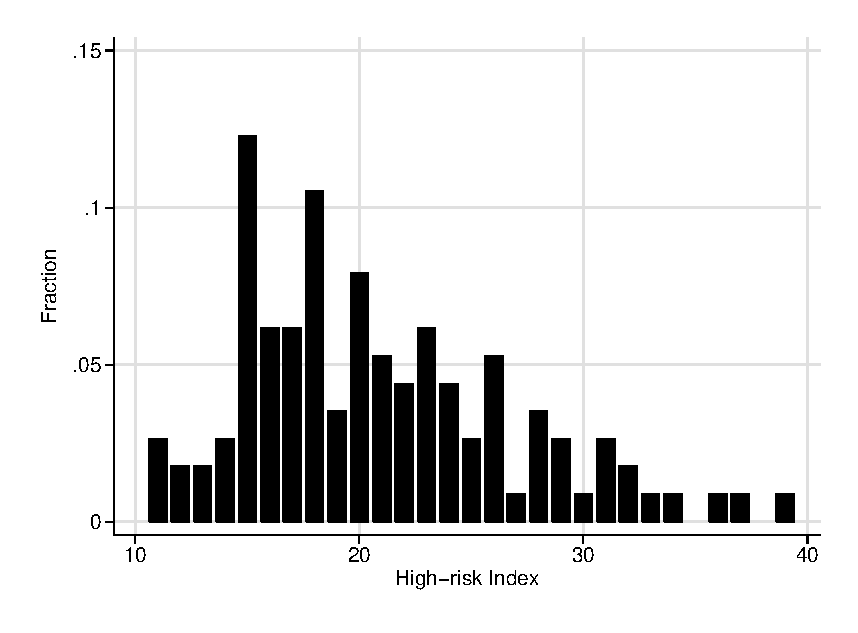
\includegraphics[width=.9\columnwidth]{output/abc_hri.eps}
\floatfoot{
\footnotesize
\noindent Note: This plot shows the distribution of the High-Risk Index (HRI) on which eligibility was based. Children were eligible if they had a score of 11 or more.}
	\end{figure}
\end{center}

\noindent Figure~\ref{figure:hridistabc} displays the distribution of the HRI among all participants. All children were substantially disadvantaged. Maternal age when the target child was born was, on average, 19.9 years. Approximately half of the mothers of both treatment and control group participants were 19 years old or younger and one third were 17 or younger.  Mean maternal IQ for both groups was approximately 85, one standard deviation below the national mean. Only 25\% of the ABC children lived with both biological parents, and more than 50\% lived with extended families in multi-generational households (61\% of treatment-group children and 56\% of control-group children).\footnote{\citet{Ramey_Campbell_1991_childreninpoverty,Campbell_Ramey_1994_CD}.}\\

\subsubsection{Randomization Protocol and Compromises} \label{appendix:randomization}

\noindent Randomization compromises throughout ABC's implementation pose a challenge when evaluating the program's effect. We discuss each case of compromise in detail in Section~\ref{section:background}. In Section~\ref{section:methodology},  we propose a methodology for adequately evaluating the program while accounting for these compromises.

\begin{center}
	\begin{figure}[H]
		\caption{Randomization Protocol and Treatment Compliance, ABC} \label{fig:abc-flow}
		\centering
		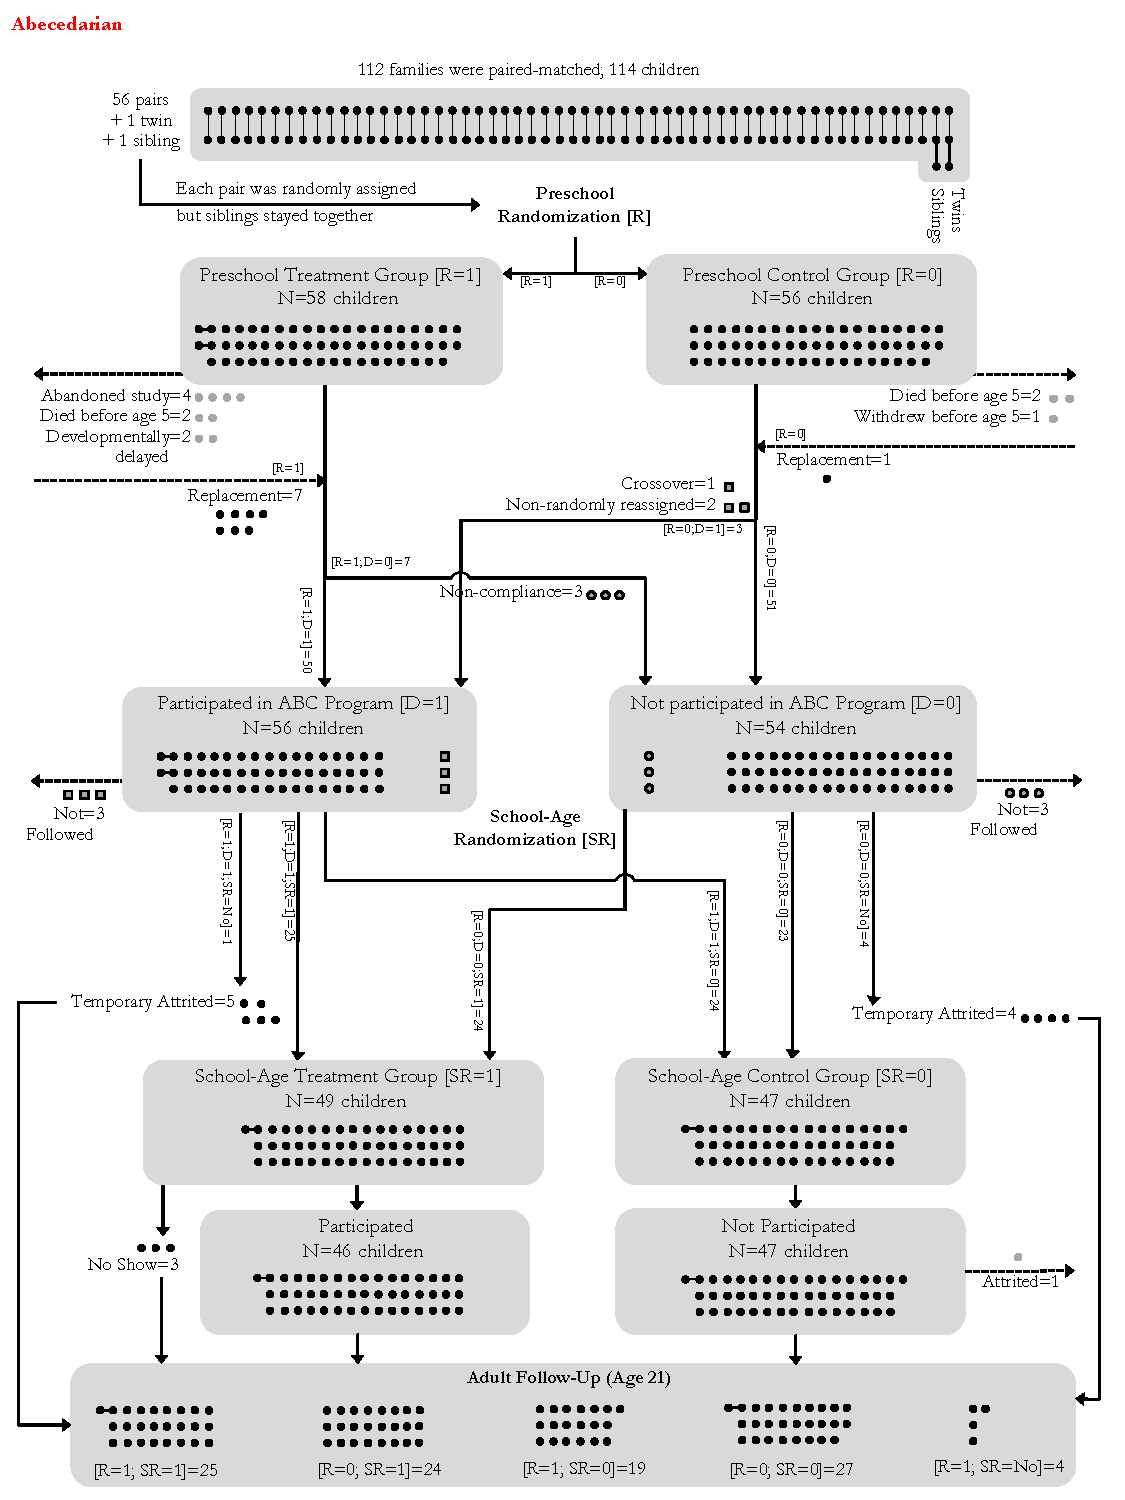
\includegraphics[width=.7\columnwidth]{output/abc_Diagram.pdf}
\floatfoot{
\footnotesize
\noindent
Sources: \cite{Ramey_Collier_etal_1976_CarolinaAbecedarianProject, Ramey_Smith_1977_AJMD,Ramey_Campbell_1979_SR,Ramey_Campbell_1984_AJMD}, internal documentation of the program, and own calculations. Note: The variable R represents randomization into treatment [R=1] or control [R=0] groups. After the original randomization, some children died or withdrew from the program early in life and were replaced. R also includes those replacements. Arrows pointing outside of the diagram indicate children who left the study permanently. The variable P represents participation in the preschool-age program. The variable SR represents randomization into the school-age program [SR=1], or out of it [SR=0]. Some children were not randomized at school age [SR=No]. We use the term temporarily attrited for children who did not participate in the study at school age, but were later interviewed in the age-21 followup.
}
	\end{figure}
\end{center}

\noindent Although most randomization compromises were at early stages, this methodology also accounts for the fact that a few individuals were not in the sample either for the second-phase randomization or for the adult-age follow-ups. The following tables test differences in observed characteristics between the treatment and control groups. We test differences both by cohort and by pooling the four cohorts. Despite the randomization compromises, we only find slight differences in observed characteristics between the children in the treatment and the control group. In Appendix~\ref{appendix:data}, we describe the sample reductions that attrition at different stages of the study generates and test potential differences between the children who were followed-up on and the children who were not.\\

\subsubsection{Program Description and Content}

\paragraph{Goals}
\noindent The original goal of treatment was to prevent mental retardation by enhancing overall development from birth,\footnote{Note that the clinical understanding of mental retardation was once associated with disadvantages that hindered early-life development \citep{Mental-Retardation_America_2004_BOOK_NYU}.} fostering school-readiness for an at-risk population. Additional curriculum goals were to (i) support language, motor, and cognitive development; (ii) minimize high-risk behaviors; and (iii) develop socio-emotional competencies considered crucial for school success including task-orientation, emotional self-expression, independence, sharing, and cooperation.\footnote{\citet{Sparling_1974_Synth_Edu_Infant_SPEECH,Ramey_Collier_etal_1976_CarolinaAbecedarianProject,Ramey-etal_2012-ABC}.} Implementation of ABC's educational treatment evolved each successive year as program staff evaluated ongoing outcome data.\footnote{ \citet{McGinness_1982_Language-Poverty-Child,Haskins_1985_CD,Finkelstein_1982_Day_Care_YC,Ramey-etal_1975_AJoMD}.}\\


\paragraph{Daily Schedule}
\noindent FPGC was open to families from 7:45 am to 5:30 pm, 5 days per week and 50 weeks per year.\footnote{\citet{Ramey_Collier_etal_1976_CarolinaAbecedarianProject}.} Children were offered free transportation to and from the center. A driver and second adult staffed each vehicle (one van and two station wagons) equipped with child safety seats.\footnote{\citet{Ramey_Campbell_1979_SR,abc2014-2015interviews}.} Data provided by FPGC indicate that approximately 65\% of treated families utilized the free transportation.\footnote{\citet{Barnett_Masse_2002_benefitcost}.} Vehicles typically arrived by 9:00 am to the center and departed around 3:45 pm.\footnote{\citet{Ramey-et-al_1977_Intro-to-ABC}.} At FPGC, treated children received breakfast, lunch, and a snack planned by a nutritionist.\footnote{ \citet{Haskins_1985_CD,Ramey-et-al_1977_Intro-to-ABC}.} Infants received iron-fortified formula  until doctors advised adding solid food. The control-group children also received an unlimited amount of iron-fortified formula.\footnote{\citet{Campbell_Conti_etal_2014_EarlyChildhoodInvestments,abc2014-2015interviews}.} Meals were catered by off-site kitchens. \\

\paragraph{Program Staff and Physical Space}
\noindent Treatment staff were recruited from the local community to promote trust in FPGC within the treatment community.\footnote{\citet{Ramey-et-al_1977_Intro-to-ABC,Feagans_1996_Childrens-Talk,abc2014-2015interviews}.} Infant and toddler caregivers and preschool teachers demonstrated varied educational backgrounds ranging from high school graduation to master's degrees. Their average professional working experience with young children was 7 years.\footnote{\citet{Ramey_McGinness_etal_1982_Abecedarianapproach}.} All classroom staff participated in extensive training and were closely observed by FPGC's academic staff, as part of a broad variety of ongoing clinical and social research related to early childhood education, psychology, and health. Child-adult ratios varied by age: 3:1 for infants up to 13 to 15 months of age; 4:1 for toddlers up to 36 months; and 5:1 or 6:1 for children aged 3 to 5 years, depending on cohort size.\footnote{\citet{Ramey-et-al_1977_Intro-to-ABC,Ramey_Campbell_1979_SR,Ramey_McGinness_etal_1982_Abecedarianapproach}.}\\

\noindent The ABC staff included a program director, a secretary, 12 to 14 teachers and assistant teachers, 3 administrative staff members, and a transportation supervisor.\footnote{\citet{Ramey-et-al_1977_Intro-to-ABC,Ramey_McGinness_etal_1982_Abecedarianapproach}.} Classroom staff included infant caregivers and preschool teachers who had an average of 7 years of experience in early childhood care at hiring. Lead caregivers and teachers had bachelor's or master's degrees. Teacher aides, recruited from the local community, held high school diplomas (at minimum) and were comparatively well-compensated in the childcare field. They remained a stable treatment component throughout the study. Classroom staff received weekly training, daily supervision, and frequent professional development from outside consultants.\footnote{\citet{Obrien-Sanders_1974_ABC-brochure,Sanders-Stokes_1979_Status-Report,Klein-Sanders_1982_Status-Report,abc2014-2015interviews}.}\\

\noindent Infant nurseries, toddler rooms, and preschool classrooms were housed on different floors of FPGC. Early reports indicate that FPGC allocated two floors to the study, but later reports indicate the use of three floors.\footnote{\citet{Ramey_Smith_1977_AJMD,Ramey_Campbell_1979_SR,Ramey_1981_Modification}.} Two infant nurseries were staffed by five adults in a suite of four adjoining rooms: two sleeping rooms contained seven cribs each, while the other two rooms were designated for activities.\footnote{ \citet{Ramey-et-al_1977_Intro-to-ABC}.} The four rooms opened into a large, shared space with feeding tables, an area for food preparation, and a couch.\footnote{\citet{Ramey_Campbell_1979_SR}.} Offices for the medical staff, along with two examining rooms and facilities for laboratory tests were located around the corner from the infant nurseries.\footnote{\citet{abc2014-2015interviews}.} Two multi-age toddler rooms were located one floor below the infant nurseries. One room served children who were 1 to 2 years old and the other served children 2 to 3 years old.\footnote{\citet{Ramey_Smith_1977_AJMD,Ramey_Campbell_1979_SR}.} 3-year-olds were housed in a closed classroom near the toddler rooms. On the lowest floor, 4-year-olds shared an open classroom with a public kindergarten program; the two classes were separated by a long, low bookcase. FPGC offered two outdoor play areas: one for toddlers and 3-year-olds, and the other for older children.\footnote{\citet{Ramey_Campbell_1979_SR,Ramey_McGinness_etal_1982_Abecedarianapproach}.}\\

\paragraph{Approach to Child Development}
%Direct from the paper
\noindent Curriculum delivery enabled a highly customized learning experience for ABC-treated children. Infant caregivers recorded child observations on progress charts and collaborated with FPGC's curriculum developers and academic researchers to rotate learning activities every 2 to 3 weeks for each treated child.\footnote{\citet{Ramey_Collier_etal_1976_CarolinaAbecedarianProject,Campbell_Ramey_1994_CD}.} Preschool rooms featured intentionally organized environments to promote pre-literacy and access to a rich set of learning tools. The full-day curriculum emphasized active learning experiences, dramatic play, and pre-academics. Frequent 1:1 or 2:1 child-adult interactions prioritized language development for social competence. For ages 3 through 5, as the cohorts approached public school entry, classroom experiences were increasingly structured  towards the development of pre-academic skills and ``socio-linguistic and communicative competence.''\footnote{\citet{Ramey-et-al_1977_Intro-to-ABC, Haskins_1985_CD, Ramey_1981_Modification, Ramey_Campbell_1979_SR, Ramey_Smith_1977_AJMD, Ramey_McGinness_etal_1982_Abecedarianapproach, Sparling_Lewis_1979_BOOKLearninggamesFirstThree,Sparling_Lewis_1984_BOOKLearningGamesThreesFours}.}\\

\noindent ABC's learning program was influenced by key developmental theorists, including Bowlby, Piaget, Vygotsky, and Tough.\footnote{\citet{Sparling_1974_Synth_Edu_Infant_SPEECH,Mcginness_1981_Developing,abc2014-2015interviews}.} All four ABC cohorts participated in curriculum developers Sparling and Lewis' ``Learningames for the First Three Years.''\footnote{ \citet{Sparling_Lewis_1979_BOOKLearninggamesFirstThree}.} The ``Learningames'' were implemented daily by infant and toddler caregivers in 1:1 child-adult interactions. Designed for use indoors and outdoors, while dressing, eating, bathing, or during play, each ``Learningames'' activity stated a developmentally-appropriate objective, the necessary materials, directions for teacher behavior, and expected child outcome.\footnote{\citet{Ramey_Campbell_1979_SR, Ramey_1981_Modification,Sparling_Lewis_1979_BOOKLearninggamesFirstThree}.}\\

\noindent Supplemental curricula for preschool rooms varied throughout the study, and included ``Cook and Learn,'' ``Bridges to Reading,'' ``Peabody Early Experiences Kit,'' ``GOAL Math Program,'' ``My Friends and Me,'' and ``Teaching all Children to Read.''\footnote{ \citet{Greenberg_Epstein_1973_BOOKBridgestoreading,Karnes1973,Dunn_Chun_etal_1976_BOOKPeabodyearlyeducation,Davis_1977_BOOKMyfriends,Wallach_1976_Teaching-All-Children}.} Packaged preschool supplemental curricula supported individual children's learning needs, and varied from year to year.\footnote{ \citet{Ramey_McGinness_etal_1982_Abecedarianapproach,Mcginness_1981_Developing,Finkelstein_1982_Day_Care_YC,Wasik_Ramey_etal_1990_CD}.}\\
%SK notes to co-authors: I'm currently waiting for info from Lynne Vernon-Feagans to potentially include a social worker to the list of staff!

\paragraph{Medical Care and Nutrition}
%Direct from the paper
ABC provided comprehensive on-site medical care because it was conducted in conjunction with a longitudinal medical research study on infectious respiratory diseases in group environments.\footnote{\citet{Henderson-et-al_1982_NEJoM}.} Treatment group children were monitored daily for signs of illness. All treated children received medical care while attending center-based childcare; the first cohort of control-group children also received medical care during the program's first year of implementation.\footnote{\citet{Ramey_Collier_etal_1976_CarolinaAbecedarianProject,Ramey_Campbell_1991_childreninpoverty,Campbell_Ramey_1994_CD}.}$^{,}$\footnote{Children in both the treatment and control groups of the first cohort received free medical care provided by ABC. The control group of the first cohort only received medical care in the first year of the program; the treatment group of the first cohort received medical care for all years of the program. In the subsequent cohorts, only children in the treatment group received free medical care provided by ABC.}\\
%Direct from the paper

\noindent Primary pediatric care was provided by a family nurse practitioner and a licensed practical nurse, both under the supervision of one pediatrician who was on continuous duty at the center.\footnote{\citet{Haskins-et-al_1978_JoPP}.} The medical staff provided regularly scheduled check-ups, immunizations, parental counseling, and initial assessment of illnesses.\footnote{\citet{Ramey-et-al_1977_Intro-to-ABC}.} The treatment group received standard check-ups when they were 2, 4, 6, 9, 12, 18, and 24 months old and annually thereafter. While in treatment, they also received the standard immunizations.\footnote{\citet{Campbell_Conti_etal_2014_EarlyChildhoodInvestments}.} A licensed practical nurse visited classrooms for up to two hours on a daily basis to monitor the children's health status.\footnote{\citet{Sanyal_Henderson_etal_1980_JoPediatrics}.} This part of treatment was free of charge to the parents. However, it was the policy of the medical staff to refer families to a community hospital for serious treatment. While ABC provided aspirin, immunizations, and basic medicines, families were responsible for purchasing any prescription medication subjects required. There is no data currently available on treatment received for serious conditions or use of prescription medication.  Infants were supplied with iron-fortified formula. Children older than 15 months of age were provided breakfast, lunch, and an
afternoon snack all planned by a nutritionist.\footnote{\citet{Campbell_Conti_etal_2014_EarlyChildhoodInvestments,abc2014-2015interviews}.} Control families received diapers for up to three years and unlimited iron-fortified bottled formula through 15 months.\footnote{\citet{Ramey_Collier_etal_1976_CarolinaAbecedarianProject,Ramey_Campbell_1979_SR}.}

\paragraph{School-age Treatment}

\noindent The ABC participants were subject to a second-phase randomization into a school-age treatment (95 subjects continued to this stage of treatment). The school-age treatment lasted for the first three years of elementary school and consisted of home visits conducted by a Home/School Resource Teacher.\footnote{\cite{Burchinal_Campbell_etal_1997_CD}.} These visits were structured to increase exposure to reading and mathematics and promote parental involvement in the learning process.\\

\noindent The curriculum was delivered through sets of activities (around 60 per year) that developed skills such as handwriting, phonics, and math facts.\footnote{\cite{Campbell-Ramey_1989_Preschool-vs-School-age}.} Teachers worked to build parental confidence as educators and provided incentives to families to comply with the treatment, such as giving gift certificates to restaurants and books for children upon the completion of activity packets. Home activities were designed at the appropriate level to promote success.\\

\noindent Teachers had graduate-level education, training in special education, \textit{or} were qualified to act as consulatants for in-school teachers to address any problems that arose.\footnote{\cite{Ramey_Campbell_1991_childreninpoverty}.} They met with parents every other week to deliver new activities for them to complete with their children and discuss the child's level of success with the previous set of activities. In addition, they helped parents with issues such as adult literacy, housing, and medical care. Thus, the teacher had a dual role as a parent educator and an advocate for the child in their educational institution.

\subsubsection{Treatment Substitution}

\noindent The families of almost $70\%$ of the control-group children enrolled their children in high-quality childcare. We refer to this phenomenon as treatment substitution; accounting for it is fundamental when evaluating the program, as we argue in Section~\ref{section:methodology}. In this appendix, we thoroughly describe the characteristics and costs of the childcare centers providing alternative treatment, in order to create a comparison with the treatment offered by ABC.\\

\noindent The centers in which most of the children in the control group took-up an alternative to the treatment ABC offered received federal subsidies and, therefore, were regulated by the Federal Interagency of Day Care Requirements (see Figure~\ref{fig:ccabc}). They were required to have trained staff who were able to implement curricula designed to enhance cognitive, social, and linguistic competence in disadvantaged children.\footnote{\citet{Burchinal_etal_1989_CD_Daycare-Pre-K-Dev}.} Thus, we consider these centers to offer high-quality center-based care.

\begin{center}
	\begin{figure}[H]
		\caption{Treatment Substitution, ABC} \label{fig:ccabc}
		\centering
		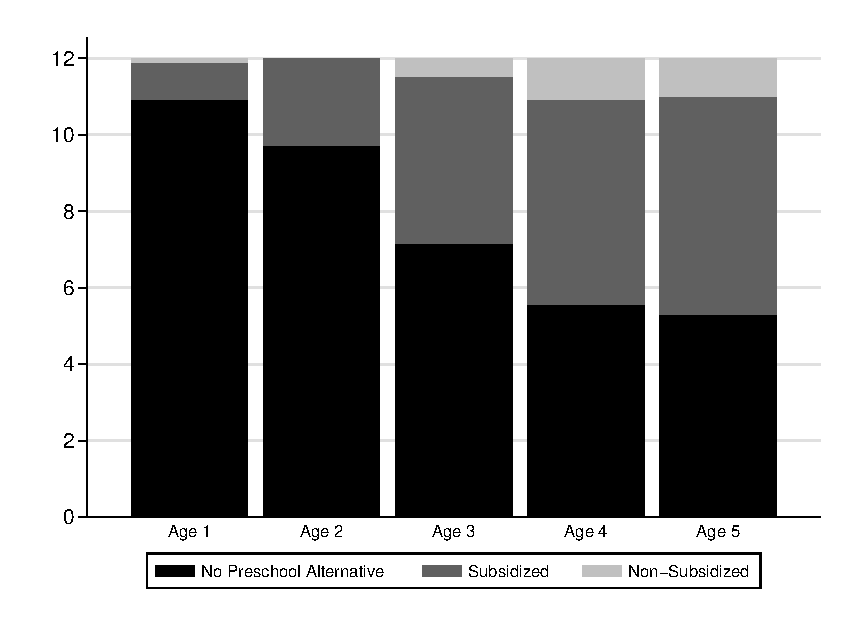
\includegraphics[width=.9\columnwidth]{output/blackwhite_CCnumber.eps}
\floatfoot{
\footnotesize
\noindent Note: This figure describes the take-up of center-based childcare by families in the control group. The vertical axis represents the average number of months per year the children of the control group spent in center-based childcare. Subsidized centers were highly regulated and, therefore, high-quality. Non-subsidized childcare services were center-based but not regulated. Other sources of childcare could have included care by parents, relatives, or non-relatives.}
	\end{figure}
\end{center}

\paragraph{Regulation}

\noindent During the ABC program, North Carolina had an active, high-quality system of public childcare for vulnerable families funded by several public programs. Examples include Title IV-A of the Social Service Administration (SSA), Aid to Families with Dependent Children (AFDC), and Title IV-B of Child Welfare Services. These funding efforts were amplified in 1975 by Title XX of the SSA, Social Services Block Grant, which was the main federal source of childcare financing in the US when ABC was active.\footnote{\citet{Robins_1988_Federal-Child-Care}.}\\

\noindent Federally funded childcare services were regulated by the Federal Interagency of Day Care Requirements (FIDCR), which defined stringent regulation for center-based programs for children between the ages of 3 and 6.\footnote{\citet{Department-of-Health_1968_DayCareRequirements}.} These requirements were enforced and childcare providers were aware of them.\footnote{\citet{Kuperman_2015_Clifford-Russell-Interview}.} Additionally, North Carolina had a mandatory licensing law for childcare facilities. This regulation only applied to centers serving children below the age of 3 while FIDCR applied to centers for older children (between the ages of 3 and 6). The relative weakness of this regulation\footnote{\citet{NCGA_1971_House-Bill-100}.} is not very relevant for our study because treatment substitution occurred mostly after age 3. Table~\ref{table:staff} compares a widely-used quality standard, the child-staff ratio, between the North Carolina and FIDCR standards and the actual ABC numbers.

%Not in main paper
\begin{table}[H]
\caption{Child-Staff Ratios for North Carolina, FIDCR, and Actual ABC Ratios}
\label{table:staff}
\begin{threeparttable}
\begin{tabular}{lccc}
\hline \hline
 &NC Standards &	&  \\
Age	& Level I & FIDCR Standards  & ABC Ratios\\ \hline
0--1	& 6:1*	&  				& 	3:1					\\
1--2	& 8:1* 	& 				&   4-5:1				\\
2--3	& 12:1* & 				& 	4-5:1				\\
3--4	& 15:1 	& 		5:1*	& 	4-5:1 				\\
4--5	& 20:1 	& 		7:1*	& 	5-6:1 				\\
5--6 & 25:1  &		7:1*	&	5-6:1				\\
\hline \hline
\end{tabular}
\begin{tablenotes}
\footnotesize
Sources: \cite{Department-of-Health_1968_DayCareRequirements,NCGA_1971_House-Bill-100,Ramey-et-al_1977_Intro-to-ABC,Ramey_Campbell_1979_SR,Ramey_McGinness_etal_1982_Abecedarianapproach} \\
Note: The starred ratios represent the ones we believe were the most relevant for ABC control-group children.
\end{tablenotes}
\end{threeparttable}
\end{table}

\paragraph{Costs}

\noindent Center-based childcare centers had a uniform rate for subsidy-eligible children, independent of which program the children were eligible for. This was mandated by the County Department of Social Services. The most common way for a child to be eligible was by belonging to a poor family with either a single mother who worked or studied or with both parents who either worked or studied. Other conditions, such as abuse risk, were also considered. Our information on the rates paid is limited, but anecdotal evidence indicates that the subsidy value for full-time center-based childcare was around \$300 at the time.\footnote{\citet{Kuperman_2015_Clifford-Russell-Interview}.} \textbf{[JLG: AZ, could you please check how often this was and the base year of these dollars?]}

\subsubsection{Data} \label{appendix:data}

In Table~\ref{tab:ecvars_1} to Table~\ref{tab:adultvars_2}, we summarize the data availability for both ABC and CARE. The data collection processes in both programs were analogous by design. For both programs, the treatment and control groups were followed into adulthood with relatively low attrition. For ABC, children were followed annually through elementary school and at ages 12, 15, 21, and 30. Health and administrative crime data were collected when the children reached their mid-30s. For CARE, the exact same follow-ups are available with the exception of the age 15 follow-up.\\

\begin{sidewaystable}[H]
\small
\caption{Early Childhood Data (Part I)}
\label{tab:ecvars_1}
\centering
\begin{adjustbox}{max width=\textwidth, max height=\textheight,keepaspectratio}
\begin{threeparttable}
\tiny
\begin{tabular}{L{3cm} C{3.5cm} C{4cm} C{1.5cm} C{1.5cm}  C{6cm}}
\toprule
\textbf{Category}	&	\textbf{Sub-Category}	&	\textbf{Description}	&	\textbf{ABC Age}  	&  \textbf{CARE Age}  & 	\textbf{Measure}	\\ \midrule
Demographics	&	Gender	&	Gender of child	&	Birth, 18, 30, 42, 54	&	 Birth, 18, 30, 42, 54	&	Demographic Interview	\\
	&	\\
	&	Race	&	Race/Cultural identity of child	&	Birth, 18, 30, 42, 54	&	 Birth, 18, 30, 42, 54	&	 Demographic Interview\\
	&	\\
	&	Birth Date	&	Date of birth of child	&	Birth, 18, 30, 42, 54	& 	Birth, 18, 30, 42, 54	&	 Demographic Interview	\\ \midrule
Cognitive Assessments	&	Language Ability	&	Auditory association, Verbal expression, etc. 	&	36, 42, 48, 54	&	30, 42, 54	&	ITPA$^{ABC}$, GPB$^{ABC}$, PLP$^{ABC}$, MSCD \\
	&	\\
	&	Intelligence Levels	&	SBIS 	&	24, 36, 48, 60	&	24, 36, 48, 60	&	SBIS	\\
	&		&	WPPSI	&	60	&	60	&	WPPSI	\\
	&		&	BSID 	&	3, 6, 9, 12, 18, 24	&	6, 12, 18, 24		&	BSID	\\
	&		&	UOSPD	&	15	&	- 	&	UOSPD$^{ABC}$	\\
	&		&	RPM	&	60	&	-	&	RPM$^{ABC}$	\\
	&	\\
	&	Quantitative	 &	BSID 	&	3, 6, 9, 12, 18, 24	&	6, 12, 18, 24		&	BSID	\\
	&		&	MSCD 	&	30, 42, 54		&	30, 42, 54	&	MSCD	\\
	&	\\
	&	Memory	&	BSID 	&	3, 6, 9, 12, 18, 24	& 	6, 12, 18, 24		&	BSID	\\
	&		&	MSCD 	&	30, 42, 54	&	30, 42, 54	&	MSCD	\\
	&	\\
	&	Motor Development	&	BSID 	&	3, 6, 9, 12, 18, 24	&	6, 12, 18, 24		&	BSID\\
	&		&	MSCD 	&	30, 42, 54	&	30, 42, 54	&	MSCD	\\
	& 	\\
	&	Critical Thinking	&	Curiosity	&	30, 36, 42, 48, 54, 60, 66, 72	& - &	Infant Behavior Inventory$^{ABC}$	\\ \midrule
Non-Cognitive Assessments	&	Social Skills	&	Positive social response	&	30, 36, 42, 48, 54, 60, 66, 72	&	6, 12, 18, 24		&	Infant Behavior Inventory$^{ABC}$, Bayley Infant Inventory$^{CARE}$	\\
	&		&	Creativity	&	30, 36, 42, 48, 54, 60, 66, 72	&	- 	&	Infant Behavior Inventory$^{ABC}$	\\
	&	\\
	&	Self-Control	&	Locus of control	&	3, 18	&	6, 18	& 	RIES	\\
	&		&	Distractibility, Attentiveness	&	30, 36, 42, 48, 54, 60, 66, 72	&	6, 12, 18, 24		&	Infant Behavior Inventory$^{ABC}$, Bayley Infant Inventory$^{CARE}$	\\
	&	\\
	&	Emotional Health	&	KRT	&	24, 36, 48, 60	&	24, 30, 36, 42, 48, 60	&	KRT	\\
	&	\\
	&	Self-Consciousness	&	Self-consciousness	&	30, 36, 42, 48, 54, 60, 66, 72	&	-	&	Infant Behavior Inventory$^{ABC}$	\\
\bottomrule
\end{tabular}
\begin{tablenotes}
\scriptsize
\item Sources: Authors' description. \\	
\item Note: This table describes the major categories of variables that were measured for ABC and CARE subjects up to age 6. ABC and CARE ages are measured in months. This is not an exhaustive list of variables, nor does it include variables from auxiliary data. Instruments or questionnaires available for only one of the studies are indicated with the superscript $^{ABC}$ or $^{CARE}$.  \textbf{Abbreviations are as follows.} ITPA: Illinois Test of Psycholinguistic Ability. GPB: Gordon Psycholinguistic Battery. PLP: Preschool Language Performance. MSCD: McCarthy Scales of Children's Development. BSID: Bayley Scales of Infant Development and Infant Behavior. UOSPD: Uzgiris-Hunt Ordinal Scales of Psychological Development. RPM: Raven's Progressive Matrices. RIES: Rotter's Internality-Externality Scale. KRT: Kohn and Rosman Test Behavior Inventory.
\end{tablenotes}
\end{threeparttable}
\end{adjustbox}
\end{sidewaystable}




\begin{sidewaystable}[H]
\small
\caption{Early Childhood Data (Part II)}
\label{tab:ecvars_2}
\centering
\begin{adjustbox}{max width=\textwidth, max height=\textheight,keepaspectratio}
\begin{threeparttable}
\tiny
\begin{tabular}{L{3cm} C{3.5cm} C{4cm} C{1.5cm} C{1.5cm}  C{6cm}}
\toprule
\textbf{Category}	&	\textbf{Sub-Category}	&	\textbf{Description}	&	\textbf{ABC Age}  	&  \textbf{CARE Age}  & 	\textbf{Measure}	\\ \midrule
Family Environment	&	Family Members	&	Number of primary caretakers	&	Birth, 18, 30, 42, 54	&	18, 30, 42, 54, 60	&	Demographic Interview	\\
	&		&	Relationship with family members, including father, mother, siblings, etc.	&	Birth, 18, 30, 42, 54	&	18, 30, 42, 54, 60	&	Demographic Interview	\\
	&		&	Number of siblings	&	Birth, 18, 30, 42, 54	&	Birth, 18, 30, 42, 54, 60	&	Demographic Interview	\\
	&		&	Marital status of parents	&	Birth, 18, 30, 42, 54	&	Birth, 18, 30, 42, 54, 60	&	Demographic Interview	\\
	&		&	Marital conflicts between parents	&	6, 18	&	Birth, 6, 18, 36	&	Demographic Interview$^{CARE}$, Parental Attitudes Research Inventory	\\
	&		& Father at home & 18, 30, 42, 54  & 18, 30, 42, 54, 60 & Demographic Interview \\
	&	\\
	&	Family Economic Environment	&	Parents' occupation	&	Birth, 18, 30, 42, 54	& 	Birth, 18, 30, 42, 54, 60		&	Demographic Interview	\\
	&								& Mother works & 18, 30, 42, 54 & 18, 30, 42, 54, 60 & Demographic Interview \\
	&		&	Source of child support	&	Birth, 18, 30, 42, 54	&	18, 30, 42, 54, 60	&	Demographic Interview	\\
	&		&	Family income	&	Birth, 18, 30, 42, 54	&	Birth, 18, 30, 42, 54, 60	&	Demographic Interview	\\
	&	\\
	&	Parents and Home Environment & Parents' authority, warmth, family conflict, etc. & 6, 18, 30, 42, 54 & 6, 12, 18, 30, 42, 54 & Parent Interview \\
	&	\\
	&	Family Social Status	&	Parents' education background	&	Birth, 18, 30, 42, 54	&	Birth, 18, 30, 42, 54, 60		&	Demographic Interview	\\
	&		&	Risk taking of family members	&	Birth	&	- 	&	Parent Interview$^{ABC}$	\\
	&	\\
	&	Family Members' Physical Health	&	Health issues of parents	&	Birth	&	Birth	&	Parent Interview	\\
	&		&	Pregnancy history	&	Birth	&	Birth	&	Parent Interview	\\ \midrule
Childcare	&	Day-care Experience	&	Time and location of day-care, Age when begin	&	Birth, 18, 30, 42, 54	&	18, 30, 42, 54	&	Demographic Interview	\\
			&						& 	Home visits &	-	&	6, 18, 30, 42, 54, 60	& Home Visit Data$^{CARE}$ \\
	&	\\
	&	Parental Care	&	Maternal warmth, Maternal involvement with child	&	6, 18, 30, 42, 54	&	6, 12, 18, 30, 42, 54	&	Home Stimulation	\\
	&		&	Provision of appropriate play materials	&	6, 18, 30, 42, 54	&	 6, 12, 18, 30, 42, 54	&	Home Stimulation	\\
	&		&	Avoidance of restriction and punishment	&	6, 18, 30, 42, 54	&	6, 12, 18, 30		&	Home Stimulation	\\
	&		&	Authoritarian control	&	6, 18, 30, 42, 54	&	6, 12, 18, 30, 36, 42, 102		&	Home Stimulation, Parental Attitudes Research Inventory	\\
	&		&	Democratic attitudes	&	6, 18	&	6, 18, 36	&	Parental Attitudes Research Inventory	\\
	&		&	Hostility and rejection	&	6, 18	&	6, 18, 36	&	Parental Attitudes Research Inventory	\\
	&		&	Parents' knowledge of childcare	&	Birth	&	-	&	Parent Interview$^{ABC}$	\\ \midrule
Physical Health	&	Growth Data	&	Height, Weight, Head circumference, etc.	&	3, 6, 9, 12, 18, 24, 36, 48, 60	&	Birth, 6, 12, 18, 24, 36, 48, 60	&	Growth Measures	\\
\bottomrule
\end{tabular}
\begin{tablenotes}
\scriptsize
\item Sources: Authors' description. \\	
\item Note: This table describes the major categories of variables that were measured for ABC and CARE subjects up to age 6. ABC and CARE ages are measured in months. This is not an exhaustive list of variables, nor does it include variables from auxiliary data.  Instruments or questionnaires available for only one of the studies are indicated with the superscript $^{ABC}$ or $^{CARE}$.
\end{tablenotes}
\end{threeparttable}
\end{adjustbox}
\end{sidewaystable}



\begin{sidewaystable}[H]
\begin{threeparttable}
\small
\caption{Childhood and Adolescence Data (Part I)} \label{tab:youthvars_1}
\centering
\tiny	
\begin{tabular}{L{3.5cm} C{3.5cm} C{5cm} C{1.5cm} C{1.5cm} C{6cm}}
\toprule
\textbf{Category}	&	\textbf{Sub-Category}	&	\textbf{Description}	&	\textbf{ABC Age}  	&  \textbf{CARE Age}  & 	\textbf{Measure}	\\ \midrule
Cognitive Assessment	&	Language Ability	&	Adaptive Language Inventory	&	6, 7, 8	&	6, 7, 8	&	Adaptive Language Inventory	\\
	&		&	Language Questionnaire	&	12	&	- 	&	Language Questionnaire$^{ABC}$	\\
	&		&	MSCD 	&	7	&	- 	&	MSCD$^{ABC}$	\\
	&	\\
	&	Intelligence Tests	&	SBIS	 &	6	&	7	&	SBIS	\\
	&		&	 WIS	&	6, 7, 8, 12, 15	&	6, 8	&	WIS	\\
	&		& Kaufman$^{CARE}$ & 	-	& 6 & Kaufman$^{CARE}$ \\
	&	\\
	&	Quantitative Skills	&	MSCD$^{ABC}$ 	&	7	&	-	&	MSCD$^{ABC}$ 	\\
	&	\\
	&	Memory	&	MSCD$^{ABC}$ 	&	7	&	-	&	MSCD$^{ABC}$	\\
	&	\\
	&	Motor Skills	&	MSCD$^{ABC}$ 	&	7	&	-	&	MSCD$^{ABC}$	\\ \midrule
Non-Cognitive Assessment	&	Interpersonal Skills	&	Gets along with people	&	6, 8, 12, 15	& 	8, 12	&	PEI, CAS, PMI$^{ABC}$, SAI$^{ABC}$, Subject Interview$^{ABC}$, Quality Rank$^{CARE}$	\\
	&		&	Relationship with the other sex	&	15	&	- 	&	 SAI$^{ABC}$, Subject What I Am Like (Harter)$^{ABC}$	\\
	&	\\
	&	Critical Thinking	&	Thinks for self, questions things	&	6, 8	 &	8, 12	&	PEI, Harter Child$^{CARE}$, CBI	\\
	&		&	Concept Attainment Kit	&	6, 7, 8	&	- 	&	Concept Attainment Kit$^{ABC}$	\\
	&	\\
	&	Self-Control	&	Distracted in class	&	6, 7, 8, 12, 15	&	12	&	SCAN$^{ABC}$, CBI, WPB$^{ABC}$, PMI$^{ABC}$, SAI$^{ABC}$, Self-Evaluation Inventory$^{ABC}$	\\
	&		&	Locus of control	&	15	&	- 	&	Nowicki-Strickland Data, Pearlin Mastery Scale$^{ABC}$	\\
	&	\\
	&	Work Ethic	&	Task Orientation	&	6, 7, 8, 12, 15	&	6, 7, 8, 9, 12 	&	SCAN$^{ABC}$, CBI, PMI$^{ABC}$		\\
	&	\\
	&	Emotional Health	&	Harms self, suicidal thoughts	&	8, 12, 15	&	8, 12	 	&	Achenbach Parent,  Subject Risk Taking Survey$^{ABC}$		\\
	&		&	Depression, anxiety, fear, etc.	&	6, 7, 8, 12, 15	&	7, 8, 9, 12	&	KRT, CAS, ETS,  Achenbach Parent	\\
	&	\\
	&	Social Activities	&	Athletic activities	&	8, 12, 15	&	8, 12		&	Achenbach Parent, SAI$^{ABC}$, Subject What I Am Like (Harter)$^{ABC}$, PEI$^{CARE}$	\\
	&		&	Participant of organizations, e.g. religions	&	8, 12, 15	&	8, 12	&	Achenbach Parent, SAI$^{ABC}$, Subject Interview$^{ABC}$	\\
	&		&	Reading list	&	12, 15	&	12	&	CAS, SAI$^{ABC}$	 \\
	&		&	TV/music	&	12, 15	&	12	&	CAS, SAI$^{ABC}$	, Television Checklist$^{ABC}$		\\
	&	\\
	&	Self-Consciousness	&	Self-conscious emotions	&	8, 12, 15	&	8, 12	&	Achenbach Parent, Subject What I Am Like (Harter)	\\ \bottomrule
	\end{tabular}
\begin{tablenotes}
\scriptsize
\item Sources: Authors' descriptions. \\
\item Note: This table describes the major categories of variables that were measured for ABC and CARE subjects at ages 6 to 18. ABC and CARE age are measured in years. This is not an exhaustive list of variables, nor does it include variables from auxiliary data.  Instruments or questionnaires available for only one of the studies are indicated with the superscript $^{ABC}$ or $^{CARE}$. \textbf{Abbreviations are as follows.}  MSCD: McCarthy Scales of Children's Development. SBIS: Stanford-Binet Intelligence Scale. WIS: Wechsler Intelligence Scale for Children. KRT: Kohn and Rosman Test Behavior Inventory. WJCA: Woodcock-Johnson Test of Cognitive Abilities. PEI: Parents as Educator Interview. CAS: Child Assessment Schedule. PMI: Psychosocial Maturity Inventory. SAI: Social Adjustment Inventory for Children and Adolescents. SCAN: Schedule of Classroom Activity Norms. CBI: Classroom Behavior Inventory. WPB: Walker Problem Behavior Checklist. ETS: Emotional/Activity/Sociability/Impulsivity Temperament Survey. FES: Family Environment Scale. PIAT: Peabody Individual Achievement Test. CAT: California Achievement Test. MARS: Mid-Adolescence Rating Scale Data.
\end{tablenotes}
\end{threeparttable}
\end{sidewaystable}

	
	
\begin{sidewaystable}[H]
\begin{threeparttable}
\small
\caption{Childhood and Adolescence Data (Part II)} \label{tab:youthvars_2}
\centering
\tiny
\begin{tabular}{L{3.5cm} C{3.5cm} C{5cm} C{1.5cm} C{1.5cm} C{6cm}}
\toprule
\textbf{Category}	&	\textbf{Sub-Category}	&	\textbf{Description}	&	\textbf{ABC Age}  	&  \textbf{CARE Age}  & 	\textbf{Measure}	\\ \midrule
Family Environment	&	Family Members	&	Number of adults in house	&	6, 8, 12, 15	&	8, 12	&	PEI, Parent Interview, Subject Person In Household$^{ABC}$		\\
	&		&	Relationship with family members, including father, mother, siblings, etc.	&	6, 8, 12, 15	&	8, 12	&	PEI, FES, SAI, Subject Interview$^{ABC}$, Adult Self Report$^{ABC}$, Parent Interview, Achenbach Parent	\\
	&		&	Number of siblings	&	6, 8, 12, 15	&	7, 8, 12	&	PEI$^{ABC}$, Parent Interview	\\
	&		&	Marital status of parents	&	6, 8, 12, 15	&	7, 8, 12	&	PEI$^{ABC}$	, Parent Interview	\\
		&		& Father at home & 18, 30, 42, 54  & 18, 30, 42, 54, 60 & Demographic Interview \\
	&	\\
	&	Parents' Education Style	&	Role of parents in education	&	6, 8	&	8, 12	&	PEI, Parent Interveiw$^{CARE}$	\\
	&		&	Parents' education beliefs \& methods&	6, 8	&	8, 12 	&	PEI, Parent Interview$^{CARE}$		\\
	&		&	Parents' aspiration \& attitudes towards child	&	6, 8, 12, 15	&	8, 12	&	PEI, Parent Interview	\\
	&	\\
	&	Family Economic Environment	&	Parents' occupation	&	6, 8, 12, 15	&	7, 8, 12	&	PEI$^{ABC}$, Parent Interview	\\
		&							& Mother works & 9 & 5, 7, 8 & Demographic Interview \\
	&		&	Source of child support	&	6, 8, 12, 15	&	7, 8, 12	&	PEI$^{ABC}$, Parent Interview	\\
	&		&	Family income	&	6, 8, 12, 15	&	7, 8, 12	&	PEI$^{ABC}$, Parent Interview	\\
	&	\\
		&	Parents and Home Environment & Parents' authority, warmth, family conflict, etc. & 8 & 8 & Parent Interview \\
	&	\\
	&	Family Social Status	&	Parents' education background	&	6, 8, 12, 15	&	7, 8, 12	&	PEI$^{ABC}$, Parent Interview	\\
	&		&	Criminal history and risk taking of family members	&	8, 12, 15	&	- 	&	Subject Taylor Life Events$^{ABC}$, Parent Interview$^{ABC}$	\\
	&	\\
	&	Family Members' Physical Health	&	Health issues of adults in house	&	8, 12, 15	&	12	&	Parent Interview, Subject Taylor Life Events$^{ABC}$	\\ 	\midrule
Academic Achievements	&	Standardized Tests	&	Reading, mathematics, and language abilities	&	6, 7, 8, 12	&	6, 8, 9,12	&	CAT$^{ABC}$, PIAT$^{ABC}$, WJCA	\\
		&	\\
	&	Performance in Schoolwork	&	Drop in grades	&	12, 15		&	12	&	CAS	\\
	&		&	Lack of interest in school	&	12, 15		&	12	&	CAS	\\
	&		&  Total years in special education & 17 & 11 & Retention and Special Services Data \\
	&		&  Total years retained in school & 17 & 11 & Retention and Special Services Data \\  \midrule
Physical Health	&	Health Issues	&	Health issues of subject	&	8, 12, 15	&	8, 12	&	Achenbach Parent, Subject Interview$^{ABC}$, Adult Self Report$^{ABC}$, PEI$^{CARE}$, Parent Interview$^{CARE}$	\\
	&	\\
	&	Growth	&	Vision, weight, height	&	8	&	8	&	Growth Data	\\
	&	\\
	&	Teenage Pregnancy	&	Teenage Pregnancy	&	15	&	- 	& Subject Interview$^{ABC}$		\\ \midrule
Social Conduct	&	Law Breaking	&	Felony, Time spent incarcerated	&	15	&	- 	&	MARS$^{ABC}$, Subject Interview$^{ABC}$	\\ \bottomrule
\end{tabular}
\begin{tablenotes}
\scriptsize
\item Sources: Authors' descriptions. \\
\item Note: This table describes the major categories of variables that were measured for ABC and CARE subjects at ages 6 to 18. ABC and CARE age are measured in years. This is not an exhaustive list of variables, nor does it include variables from auxiliary data.  Instruments or questionnaires available for only one of the studies are indicated with the superscript $^{ABC}$ or $^{CARE}$. \textbf{Abbreviations are as follows.}  MSCD: McCarthy Scales of Children's Development. SBIS: Stanford-Binet Intelligence Scale. WIS: Wechsler Intelligence Scale for Children. KRT: Kohn and Rosman Test Behavior Inventory. WJCA: Woodcock-Johnson Test of Cognitive Abilities. PEI: Parents as Educator Interview. CAS: Child Assessment Schedule. PMI: Psychosocial Maturity Inventory. SAI: Social Adjustment Inventory for Children and Adolescents. SCAN: Schedule of Classroom Activity Norms. CBI: Classroom Behavior Inventory. WPB: Walker Problem Behavior Checklist. ETS: Emotional/Activity/Sociability/Impulsivity Temperament Survey. FES: Family Environment Scale. PIAT: Peabody Individual Achievement Test. CAT: California Achievement Test. MARS: Mid-Adolescence Rating Scale Data.
\end{tablenotes}
\end{threeparttable}
\end{sidewaystable}

\begin{sidewaystable}[H]							
\begin{threeparttable}								
\small										
\caption{Adulthood Data (Part I)} \label{tab:adultvars_1}						\centering										
\scriptsize										
\begin{tabular}{L{3.5cm} C{3.5cm} C{5cm} C{1.5cm} C{1.8cm} C{6cm}}										
\toprule
\textbf{Category}	&	\textbf{Sub-Category}	&	\textbf{Description}	&	\textbf{ABC Age}  	&  \textbf{CARE Age}  & 	\textbf{Measure}	\\ \midrule
Cognitive Assessments   	&	       Intelligence Tests      	&	       WIS     	&	21	&	-	&	       WIS     \\
\midrule										
Non-Cognitive Assessment        	&	       Interpersonal Skills    	&	       Gets along with people  	&	       21, 30  	&	-	&	       Subject Interview   \\
\\										
        	&	       Self-Control    	&	       Locus of control        	&	       21, 30  	&	-	&	       Nowicki-Strickland Data$^{ABC}$, Pearlin Mastery Scale$^{ABC}$  \\
        	&	               	&	       Proud of working, interest in working   	&	       21, 30  	&	21, 30	&	       Job Satisfaction Survey$^{ABC}$, Subject Interview       \\
\\										
        	&	       Emotional Health        	&	       Harms self, suicidal thoughts,	&	21	&	21	&	       Achenbach,  Subject Risk Taking Survey   \\
        	&	               	&	       depression, anxiety, fear, etc. 	&	       21, 30  	&	21, 30	&	       KRT, Achenbach Parent,  CAS, Brief Symptom Inventory, ETS\\
\\										
        	&	       Social Activities       	&	       Athletic activities     	&	21	&	-	&	       Achenbach,  \\
        	&	               	&	       Participant of organizations, e.g. religions    	&	       21, 30  	&	21, 30	&	       Achenbach, Subject Interview        \\
\midrule										
Family Environment      	&	       Family Members  	&	       Number of adults in house       	&	21	&	-	&	       Parent Interview$^{ABC}$ , Subject Interview    \\
        	&	               	&	       Relationship with family members, including father, mother, siblings, etc.      	&	       21, 30  	&	30	&	      Parent Interview, Achenbach$^{ABC}$, Subject Interview, Adult Self Report \\
        	&	               	&	       Number of siblings      	&	       21, 30  	&	30	&	       Parent Interview$^{ABC}$ , Subject Interview    \\
        	&	               	&	       Marital status of parents       	&	21	&	-	&	       Parent Interview$^{ABC}$ , Subject Interview    \\
        	&	               	&	       Number of children, childcare basics    	&	       21, 30  	&	30	&	       Subject Interview, Childcare Questionnaire      \\
\\										
        	&	       Family Economic Environment     	&	       Parents' occupation     	&	21	&	-	&	       Parent Interview$^{ABC}$ , Subject Interview    \\
        	&	               	&	       Source of child support 	&	21	&	30	&	       Parent Interview$^{ABC}$ , Subject Interview    \\
        	&	               	&	       Family income   	&	21	&	30	&	       Parent Interview$^{ABC}$ , Subject Interview    \\
\\										
        	&	       Family Members and Children	&	Relationship quality, family health issues, attitude toward child learning	&	30	&	30	&	       Parent Interview, Taylor Life Events$^{ABC}$, Child Health Questionnaire, PEI    \\
\\										
        	&	       Marital Status  	&	       Marital status, spouse income       	&	       21, 30  	&	21, 30	&	       Subject Interview       \\
        	&	               	&	       Spouse details, marriage history	&	       21, 30  	&	30	&	       Subject Interview       \\
        	&	               	&	       Relationship with spouse        	&	       21, 30  	&	30	&	       Subject Interview, Adult Self Report    \\
\\										
 Achievement   	&	       Education Level 	&	       Years in school, plans for future education      	&	       21, 30  	&	       21, 30  	&	       Subject Interview, Adult Self Report    \\
        	&	               	&	       College type, certificate earned        	&	       21, 30  	&	       21, 30  	&	       Subject Interview, Adult Self Report    \\
	&	Achievement Test	&	       WJCA    	&	       21, 30  	&	-	&	       WJCA    \\
	&		&							
        \\ \bottomrule							
\end{tabular}										
\begin{tablenotes}									
\scriptsize										
\item Sources: Authors' description. \\				
\item Note: This table describes the major categories of variables that were measured for ABC and CARE subjects at ages 21 and 30. ABC and CARE age are measured in years. This is not an exhaustive list of variables, nor does it include variables from auxiliary data. Instruments or questionnaires available for only one of the studies are indicated with the superscript $^{ABC}$ or $^{CARE}$. \textbf{Abbreviations are as follows.} KRT: Kohn and Rosman Test Behavior Inventory. CAS: Child Assessment Schedule. ETS: Emotional/Activity/Sociability/Impulsivity Temperament Survey. WIS: Wechsler Adult Intelligence Scale. WJCA: Woodcock-Johnson Test of Cognitive Abilities. PEI: Parents as Educator Interview.		\end{tablenotes}									
\end{threeparttable}								
\end{sidewaystable}																			


\begin{sidewaystable}[H]
\begin{threeparttable}
\small
\caption{Adulthood Data (Part II)} \label{tab:adultvars_2}
\centering
\scriptsize
\begin{tabular}{L{3.5cm} C{3.5cm} C{5cm} C{1.5cm} C{1.8cm} C{6cm}}
\toprule
\textbf{Category}	&	\textbf{Sub-Category}	&	\textbf{Description}	&	\textbf{ABC Age}  	&  \textbf{CARE Age}  & 	\textbf{Measure}	\\ \midrule
Physical Health	&	Health Insurance	&	Covered by health insurance	&	21, 30	&	21, 30	&	Subject Interview	\\
\\											
	&	Health Issues	&	Health conditions, diseases, regular checkups and tests, mental health	&	21, 30	&	21	&	Brief Symptom Inventory, Subject Interview, Adult Self Report	\\
\midrule											
Social Conduct	&	Risk Taking	&	Smoking, drinking, carry gun, fight, drug use	&	21, 30	&	21, 30	&	Subject Risk Taking Survey, Adult Self Report	\\
\\											
	&	Law Breaking	&	Felony, Time spent incarcerated	&	21	&	21, 30	& Subject Interview	\\
\midrule											
Economic Status	&	Living Circumstances	&	Number of rooms	&	21, 30	&	21, 30	&	Subject Interview	\\
	&		&	Own or rent apartment	&	21, 30	&	21	&	Subject Interview	\\
	&		&	Number living in same domicile	&	21, 30	&	21	&	Subject Interview	\\
\\											
	&	Working Condition	&	Currently employed	&	21, 30	&	21, 30	&	Subject Interview	\\
	&		&	Job title	&	21, 30	&	21, 30	&	Subject Interview, Adult Self Report	\\
	&		&	Job category	&	21, 30	&	21, 30	&	Subject Interview, Adult Self Report	\\
	&		&	Hours	&	21, 30	&	21, 30	&	Subject Interview, Adult Self Report	\\
	&		&	Satisfied with current job	&	21, 30	&	21, 30	&	Subject Interview, Subject What I Am Like (Harter), Adult Self Report	\\
\\											
	&	Transportation	&	Own reliable transportation	&	21, 30	&	21	&	Subject Interview, Adult Self Report	\\
	&		&	Public transportation	&	21, 30	&	21	&	Subject Interview, Adult Self Report	\\
\\											
	&	Income	&	Income from job	&	21, 30	&	21, 30	&	Subject Interview, Adult Self Report	\\
	&		&	Income from welfare programs	&	21, 30	&	30	&	Subject Interview, Adult Self Report	\\
	&		&	Income from investment	&	21, 30	&	-	&	Subject Interview, Adult Self Report	\\										
 \bottomrule
\end{tabular}										
\begin{tablenotes}									
\scriptsize											
\item Sources: Authors' description. \\				
\item Note: This table describes the major categories of variables that were measured for ABC and CARE subjects at ages 21 and 30. ABC and CARE age are measured in years. This is not an exhaustive list of variables, nor does it include variables from auxiliary data. Instruments or questionnaires available for only one of the studies are indicated with the superscript $^{ABC}$ or $^{CARE}$.			
\end{tablenotes}									
\end{threeparttable}								
\end{sidewaystable}											


\begin{figure}[H]
\caption{Attrition by Age} \label{fig:attrition}
    \centering
  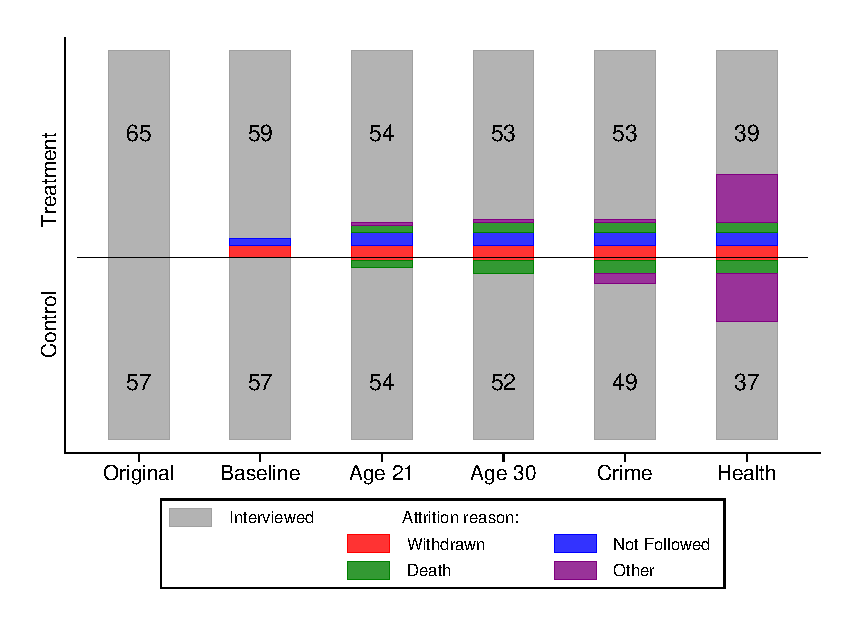
\includegraphics[width=.9\columnwidth]{output/abc_attrition.eps}
  \floatfoot{
\footnotesize
Note: This plot shows the number of participants, by experimental group, for whom there exists data at the periods of data collection. The children who withdrew from the study did so due to several reasons, such as adoption. Children were not followed if they were found to be biologically retarded after randomization. The numbers in the bars indicate the number of individuals who were interviewed during that phase of data collection. The original sample was measured after randomization but before the start of the program, the baseline sample was measured at the start of the program, and the health sample was collected at age 34.
}
\end{figure}

\noindent Attrition was low, as displayed in Figure \ref{fig:attrition}. Information is available on 100 children in the age 30 follow-up. Figure~\ref{fig:abc-flow} describes the flow of retention through all follow-ups. Additionally, 88 participants (45 from the control group and 43 from the treatment group) consented to release their criminal records and 70 participants (31 from the control group and 39 from the treatment group) released information on a full-range biomedical sweep. The data include measures such as prevalence of diabetes and high blood pressure, waist-to-hip ratio, height, weight, and cholesterol levels.\\ 

\noindent In the following set of tables, we compare the observed, baseline characteristics between the first-stage control and treatment groups, which are the main groups we analyze, at different stages of the data collection follow-ups. For each observed characteristic, we present the bootstrapped $p$-value associated with the standard $t$-test. We also present the bootstrapped, step-down $p$-value on jointly testing the difference in observed characteristics across the two blocks of variables separated by the horizontal line \citep{Lehmann_Romano_2005_testing}.\\

\noindent First, we compare the first-phase treatment and control groups on baseline characteristics. 

\begin{table}[H]
\captionsetup{singlelinecheck=false,justification=centering}
\caption{First-phase Treatment vs. Control Groups \label{tab:baseline}}

  \begin{threeparttable}
  \begin{tabular}{cccccccc}
  \hline\hline

     &  & \scriptsize{Control} & \scriptsize{Treated} & \scriptsize{Control} & \scriptsize{Treated} & \mc{2}{c}{\scriptsize{$p$-value}} \\  

    \scriptsize{Variable} & \scriptsize{Age} & \scriptsize{Obs.} & \scriptsize{Obs.} & \scriptsize{Mean} & \scriptsize{Mean} & \scriptsize{Single $H_0$} & \scriptsize{Multiple $H_0$} \\ 
    \hline  

    \mc{1}{l}{\scriptsize{Male}} & \mc{1}{c}{\scriptsize{0}} & \mc{1}{c}{\scriptsize{57}} & \mc{1}{c}{\scriptsize{59}} & \mc{1}{c}{\scriptsize{0.438}} & \mc{1}{c}{\scriptsize{0.489}} & \mc{1}{c}{\scriptsize{(0.580)}} & \mc{1}{c}{\scriptsize{(0.700)}} \\  

    \mc{1}{l}{\scriptsize{Birth Weight}} & \mc{1}{c}{\scriptsize{0}} & \mc{1}{c}{\scriptsize{56}} & \mc{1}{c}{\scriptsize{58}} & \mc{1}{c}{\scriptsize{7.191}} & \mc{1}{c}{\scriptsize{6.829}} & \mc{1}{c}{\scriptsize{(0.130)}} & \mc{1}{c}{\scriptsize{(0.205)}} \\  

    \mc{1}{l}{\scriptsize{No. Siblings in Household}} & \mc{1}{c}{\scriptsize{0}} & \mc{1}{c}{\scriptsize{57}} & \mc{1}{c}{\scriptsize{59}} & \mc{1}{c}{\scriptsize{0.750}} & \mc{1}{c}{\scriptsize{0.516}} & \mc{1}{c}{\scriptsize{(0.245)}} & \mc{1}{c}{\scriptsize{(0.425)}} \\  

    \mc{1}{l}{\scriptsize{Birth Year}} & \mc{1}{c}{\scriptsize{0}} & \mc{1}{c}{\scriptsize{57}} & \mc{1}{c}{\scriptsize{59}} & \mc{1}{c}{\scriptsize{1974}} & \mc{1}{c}{\scriptsize{1974}} & \mc{1}{c}{\scriptsize{(0.785)}} & \mc{1}{c}{\scriptsize{(0.865)}} \\ 
    \hline  

    \mc{1}{l}{\scriptsize{Mother's Education}} & \mc{1}{c}{\scriptsize{0}} & \mc{1}{c}{\scriptsize{57}} & \mc{1}{c}{\scriptsize{59}} & \mc{1}{c}{\scriptsize{9.864}} & \mc{1}{c}{\scriptsize{10.505}} & \mc{1}{c}{\scriptsize{\textbf{(0.050)}}} & \mc{1}{c}{\scriptsize{\textbf{(0.090)}}} \\  

    \mc{1}{l}{\scriptsize{Mother's Age}} & \mc{1}{c}{\scriptsize{0}} & \mc{1}{c}{\scriptsize{57}} & \mc{1}{c}{\scriptsize{59}} & \mc{1}{c}{\scriptsize{20.103}} & \mc{1}{c}{\scriptsize{19.564}} & \mc{1}{c}{\scriptsize{(0.555)}} & \mc{1}{c}{\scriptsize{(0.665)}} \\  

    \mc{1}{l}{\scriptsize{Parental Income}} & \mc{1}{c}{\scriptsize{0}} & \mc{1}{c}{\scriptsize{57}} & \mc{1}{c}{\scriptsize{58}} & \mc{1}{c}{\scriptsize{6,211}} & \mc{1}{c}{\scriptsize{7,019}} & \mc{1}{c}{\scriptsize{(0.645)}} & \mc{1}{c}{\scriptsize{(0.720)}} \\  

    \mc{1}{l}{\scriptsize{Mother's IQ}} & \mc{1}{c}{\scriptsize{0}} & \mc{1}{c}{\scriptsize{57}} & \mc{1}{c}{\scriptsize{59}} & \mc{1}{c}{\scriptsize{83.419}} & \mc{1}{c}{\scriptsize{85.393}} & \mc{1}{c}{\scriptsize{(0.360)}} & \mc{1}{c}{\scriptsize{(0.510)}} \\  

    \mc{1}{l}{\scriptsize{Father at Home}} & \mc{1}{c}{\scriptsize{0}} & \mc{1}{c}{\scriptsize{57}} & \mc{1}{c}{\scriptsize{59}} & \mc{1}{c}{\scriptsize{0.346}} & \mc{1}{c}{\scriptsize{0.223}} & \mc{1}{c}{\scriptsize{(0.135)}} & \mc{1}{c}{\scriptsize{(0.270)}} \\  

  \hline\hline
  \end{tabular}
    \begin{tablenotes}
    \scriptsize
    \item 
    Note: This table shows the balance in observed characteristics between the treatment and control groups at baseline.
    For each characteristic, we present the $p$-value from a single hypothesis test.
    We also present the $p$-values from multiple testing, where we collectively test the
    baseline characteristics within the blocks separated by the horizontal line.
    Both $p$-values are two-sided and non-parametric. We construct them 
    based on 1,000 re-draws of the full sample. The estimates we display are the means of 
    the empirical bootstrap distribution. 
    
    \end{tablenotes}
  \end{threeparttable}

\end{table}

\noindent Second, we present the same exercise for each of the four cohorts ABC served.

\begin{table}[H]
\captionsetup{singlelinecheck=false,justification=centering}
\caption{First-phase Treatment vs. Control Groups, ABC Cohort 1 \label{tab:baseline_coh1}}

  \begin{threeparttable}
  \begin{tabular}{cccccccc}
  \toprule

     &  & \scriptsize{Control} & \scriptsize{Treated} & \scriptsize{Control} & \scriptsize{Treated} & \mc{2}{c}{\scriptsize{$p$-value}} \\  

    \scriptsize{Variable} & \scriptsize{Age} & \scriptsize{Obs.} & \scriptsize{Obs.} & \scriptsize{Mean} & \scriptsize{Mean} & \scriptsize{Single $H_0$} & \scriptsize{Multiple $H_0$} \\ 
    \midrule  

    \mc{1}{l}{\scriptsize{Male}} & \mc{1}{c}{\scriptsize{0}} & \mc{1}{c}{\scriptsize{14}} & \mc{1}{c}{\scriptsize{14}} & \mc{1}{c}{\scriptsize{0.348}} & \mc{1}{c}{\scriptsize{0.286}} & \mc{1}{c}{\scriptsize{(0.730)}} & \mc{1}{c}{\scriptsize{(0.738)}} \\  

    \mc{1}{l}{\scriptsize{Birth Weight}} & \mc{1}{c}{\scriptsize{0}} & \mc{1}{c}{\scriptsize{14}} & \mc{1}{c}{\scriptsize{13}} & \mc{1}{c}{\scriptsize{6.755}} & \mc{1}{c}{\scriptsize{6.491}} & \mc{1}{c}{\scriptsize{(0.550)}} & \mc{1}{c}{\scriptsize{(0.655)}} \\  

    \mc{1}{l}{\scriptsize{No. Siblings in Household}} & \mc{1}{c}{\scriptsize{0}} & \mc{1}{c}{\scriptsize{14}} & \mc{1}{c}{\scriptsize{14}} & \mc{1}{c}{\scriptsize{1.741}} & \mc{1}{c}{\scriptsize{0.606}} & \mc{1}{c}{\scriptsize{\textbf{(0.035)}}} & \mc{1}{c}{\scriptsize{\textbf{(0.085)}}} \\  

    \mc{1}{l}{\scriptsize{Birth Year}} & \mc{1}{c}{\scriptsize{0}} & \mc{1}{c}{\scriptsize{14}} & \mc{1}{c}{\scriptsize{14}} & \mc{1}{c}{\scriptsize{1972}} & \mc{1}{c}{\scriptsize{1972}} & \mc{1}{c}{\scriptsize{(0.240)}} & \mc{1}{c}{\scriptsize{(0.350)}} \\ 
    \midrule 

    \mc{1}{l}{\scriptsize{Mother's Education}} & \mc{1}{c}{\scriptsize{0}} & \mc{1}{c}{\scriptsize{14}} & \mc{1}{c}{\scriptsize{14}} & \mc{1}{c}{\scriptsize{9.885}} & \mc{1}{c}{\scriptsize{10.561}} & \mc{1}{c}{\scriptsize{(0.265)}} & \mc{1}{c}{\scriptsize{(0.480)}} \\  

    \mc{1}{l}{\scriptsize{Mother's Age}} & \mc{1}{c}{\scriptsize{0}} & \mc{1}{c}{\scriptsize{14}} & \mc{1}{c}{\scriptsize{14}} & \mc{1}{c}{\scriptsize{23.869}} & \mc{1}{c}{\scriptsize{19.552}} & \mc{1}{c}{\scriptsize{\textbf{(0.050)}}} & \mc{1}{c}{\scriptsize{(0.135)}} \\  

    \mc{1}{l}{\scriptsize{Mother Employed}} & \mc{1}{c}{\scriptsize{0}} & \mc{1}{c}{\scriptsize{14}} & \mc{1}{c}{\scriptsize{14}} & \mc{1}{c}{\scriptsize{0.152}} & \mc{1}{c}{\scriptsize{0.205}} & \mc{1}{c}{\scriptsize{(0.695)}} & \mc{1}{c}{\scriptsize{(0.895)}} \\  

    \mc{1}{l}{\scriptsize{Parental Income}} & \mc{1}{c}{\scriptsize{0}} & \mc{1}{c}{\scriptsize{14}} & \mc{1}{c}{\scriptsize{13}} & \mc{1}{c}{\scriptsize{7,164}} & \mc{1}{c}{\scriptsize{8,298}} & \mc{1}{c}{\scriptsize{(0.755)}} & \mc{1}{c}{\scriptsize{(0.910)}} \\  

    \mc{1}{l}{\scriptsize{Mother's IQ}} & \mc{1}{c}{\scriptsize{0}} & \mc{1}{c}{\scriptsize{14}} & \mc{1}{c}{\scriptsize{14}} & \mc{1}{c}{\scriptsize{76.042}} & \mc{1}{c}{\scriptsize{81.108}} & \mc{1}{c}{\scriptsize{(0.270)}} & \mc{1}{c}{\scriptsize{(0.485)}} \\  

    \mc{1}{l}{\scriptsize{Father at Home}} & \mc{1}{c}{\scriptsize{0}} & \mc{1}{c}{\scriptsize{14}} & \mc{1}{c}{\scriptsize{14}} & \mc{1}{c}{\scriptsize{0.559}} & \mc{1}{c}{\scriptsize{0.368}} & \mc{1}{c}{\scriptsize{(0.340)}} & \mc{1}{c}{\scriptsize{(0.493)}} \\  

  \bottomrule
  \end{tabular}
    \begin{tablenotes}
    \scriptsize
    \item 
    Note: This table shows the balance in observed characteristics between the treatment and control groups in ABC at baseline for cohort 1.
    For each characteristic, we present the $p$-value from a single hypothesis test.
    We also present the $p$-values from multiple hypothesis testing, where we collectively test the
    baseline characteristics within the blocks separated by the horizontal line.
    Both $p$-values are two-sided and non-parametric. We construct them 
    based on 200 re-draws of the full sample.
    
    \end{tablenotes}
  \end{threeparttable}

\end{table}

\begin{table}[H]
\captionsetup{singlelinecheck=false,justification=centering}
\caption{First-phase Treatment vs. Control Groups, ABC Cohort 2 \label{tab:baseline_coh2}}

  \begin{threeparttable}
  \begin{tabular}{cccccccc}
  \toprule

     &  & \scriptsize{Control} & \scriptsize{Treated} & \scriptsize{Control} & \scriptsize{Treated} & \mc{2}{c}{\scriptsize{$p$-value}} \\  

    \scriptsize{Variable} & \scriptsize{Age} & \scriptsize{Obs.} & \scriptsize{Obs.} & \scriptsize{Mean} & \scriptsize{Mean} & \scriptsize{Single $H_0$} & \scriptsize{Multiple $H_0$} \\ 
    \midrule

    \mc{1}{l}{\scriptsize{Male}} & \mc{1}{c}{\scriptsize{0}} & \mc{1}{c}{\scriptsize{13}} & \mc{1}{c}{\scriptsize{16}} & \mc{1}{c}{\scriptsize{0.457}} & \mc{1}{c}{\scriptsize{0.503}} & \mc{1}{c}{\scriptsize{(0.805)}} & \mc{1}{c}{\scriptsize{(0.875)}} \\  

    \mc{1}{l}{\scriptsize{Birth Weight}} & \mc{1}{c}{\scriptsize{0}} & \mc{1}{c}{\scriptsize{13}} & \mc{1}{c}{\scriptsize{16}} & \mc{1}{c}{\scriptsize{7.256}} & \mc{1}{c}{\scriptsize{6.534}} & \mc{1}{c}{\scriptsize{(0.160)}} & \mc{1}{c}{\scriptsize{(0.270)}} \\  

    \mc{1}{l}{\scriptsize{No. Siblings in Household}} & \mc{1}{c}{\scriptsize{0}} & \mc{1}{c}{\scriptsize{13}} & \mc{1}{c}{\scriptsize{16}} & \mc{1}{c}{\scriptsize{0.388}} & \mc{1}{c}{\scriptsize{0.316}} & \mc{1}{c}{\scriptsize{(0.755)}} & \mc{1}{c}{\scriptsize{(0.835)}} \\  

    \mc{1}{l}{\scriptsize{Birth Year}} & \mc{1}{c}{\scriptsize{0}} & \mc{1}{c}{\scriptsize{13}} & \mc{1}{c}{\scriptsize{16}} & \mc{1}{c}{\scriptsize{1973}} & \mc{1}{c}{\scriptsize{1973}} & \mc{1}{c}{\scriptsize{(0.850)}} & \mc{1}{c}{\scriptsize{(0.925)}} \\ 
    \midrule  

    \mc{1}{l}{\scriptsize{Mother's Education}} & \mc{1}{c}{\scriptsize{0}} & \mc{1}{c}{\scriptsize{13}} & \mc{1}{c}{\scriptsize{16}} & \mc{1}{c}{\scriptsize{10.225}} & \mc{1}{c}{\scriptsize{10.307}} & \mc{1}{c}{\scriptsize{(0.885)}} & \mc{1}{c}{\scriptsize{(0.940)}} \\  

    \mc{1}{l}{\scriptsize{Mother's Age}} & \mc{1}{c}{\scriptsize{0}} & \mc{1}{c}{\scriptsize{13}} & \mc{1}{c}{\scriptsize{16}} & \mc{1}{c}{\scriptsize{18.446}} & \mc{1}{c}{\scriptsize{17.637}} & \mc{1}{c}{\scriptsize{(0.380)}} & \mc{1}{c}{\scriptsize{(0.630)}} \\  

    \mc{1}{l}{\scriptsize{Mother Employed}} & \mc{1}{c}{\scriptsize{0}} & \mc{1}{c}{\scriptsize{13}} & \mc{1}{c}{\scriptsize{16}} & \mc{1}{c}{\scriptsize{0.307}} & \mc{1}{c}{\scriptsize{0.248}} & \mc{1}{c}{\scriptsize{(0.690)}} & \mc{1}{c}{\scriptsize{(0.850)}} \\  

    \mc{1}{l}{\scriptsize{Parental Income}} & \mc{1}{c}{\scriptsize{0}} & \mc{1}{c}{\scriptsize{13}} & \mc{1}{c}{\scriptsize{16}} & \mc{1}{c}{\scriptsize{5,398}} & \mc{1}{c}{\scriptsize{4,427}} & \mc{1}{c}{\scriptsize{(0.790)}} & \mc{1}{c}{\scriptsize{(0.880)}} \\  

    \mc{1}{l}{\scriptsize{Mother's IQ}} & \mc{1}{c}{\scriptsize{0}} & \mc{1}{c}{\scriptsize{13}} & \mc{1}{c}{\scriptsize{16}} & \mc{1}{c}{\scriptsize{86.873}} & \mc{1}{c}{\scriptsize{85.597}} & \mc{1}{c}{\scriptsize{(0.730)}} & \mc{1}{c}{\scriptsize{(0.855)}} \\  

    \mc{1}{l}{\scriptsize{Father at Home}} & \mc{1}{c}{\scriptsize{0}} & \mc{1}{c}{\scriptsize{13}} & \mc{1}{c}{\scriptsize{16}} & \mc{1}{c}{\scriptsize{0.220}} & \mc{1}{c}{\scriptsize{0.183}} & \mc{1}{c}{\scriptsize{(0.790)}} & \mc{1}{c}{\scriptsize{(0.895)}} \\  

  \bottomrule
  \end{tabular}
    \begin{tablenotes}
    \scriptsize
    \item 
    Note: This table shows the balance in observed characteristics between the treatment and control groups in ABC at baseline for cohort 2.
    For each characteristic, we present the $p$-value from a single hypothesis test.
    We also present the $p$-values from multiple hypothesis testing, where we collectively test the
    baseline characteristics within the blocks separated by the horizontal line.
    Both $p$-values are two-sided and non-parametric. We construct them 
    based on 200 re-draws of the full sample.
    
    \end{tablenotes}
  \end{threeparttable}

\end{table}

\begin{table}[H]
\captionsetup{singlelinecheck=false,justification=centering}
\caption{First-phase Treatment vs. Control Groups, ABC Cohort 3 \label{tab:baseline_coh3}}

  \begin{threeparttable}
  \begin{tabular}{cccccccc}
  \hline\hline

     &  & \scriptsize{Control} & \scriptsize{Treated} & \scriptsize{Control} & \scriptsize{Treated} & \mc{2}{c}{\scriptsize{$p$-value}} \\  

    \scriptsize{Variable} & \scriptsize{Age} & \scriptsize{Obs.} & \scriptsize{Obs.} & \scriptsize{Mean} & \scriptsize{Mean} & \scriptsize{Single $H_0$} & \scriptsize{Multiple $H_0$} \\ 
    \hline  

    \mc{1}{l}{\scriptsize{Male}} & \mc{1}{c}{\scriptsize{0}} & \mc{1}{c}{\scriptsize{14}} & \mc{1}{c}{\scriptsize{15}} & \mc{1}{c}{\scriptsize{0.376}} & \mc{1}{c}{\scriptsize{0.596}} & \mc{1}{c}{\scriptsize{(0.265)}} & \mc{1}{c}{\scriptsize{(0.320)}} \\  

    \mc{1}{l}{\scriptsize{Birth Weight}} & \mc{1}{c}{\scriptsize{0}} & \mc{1}{c}{\scriptsize{14}} & \mc{1}{c}{\scriptsize{15}} & \mc{1}{c}{\scriptsize{7.424}} & \mc{1}{c}{\scriptsize{7.138}} & \mc{1}{c}{\scriptsize{(0.470)}} & \mc{1}{c}{\scriptsize{(0.730)}} \\  

    \mc{1}{l}{\scriptsize{No. Siblings in Household}} & \mc{1}{c}{\scriptsize{0}} & \mc{1}{c}{\scriptsize{14}} & \mc{1}{c}{\scriptsize{15}} & \mc{1}{c}{\scriptsize{0.423}} & \mc{1}{c}{\scriptsize{0.203}} & \mc{1}{c}{\scriptsize{(0.385)}} & \mc{1}{c}{\scriptsize{(0.645)}} \\  

    \mc{1}{l}{\scriptsize{Birth Year}} & \mc{1}{c}{\scriptsize{0}} & \mc{1}{c}{\scriptsize{14}} & \mc{1}{c}{\scriptsize{15}} & \mc{1}{c}{\scriptsize{1975}} & \mc{1}{c}{\scriptsize{1975}} & \mc{1}{c}{\scriptsize{(0.510)}} & \mc{1}{c}{\scriptsize{(0.520)}} \\ 
    \hline  

    \mc{1}{l}{\scriptsize{Mother's Education}} & \mc{1}{c}{\scriptsize{0}} & \mc{1}{c}{\scriptsize{14}} & \mc{1}{c}{\scriptsize{15}} & \mc{1}{c}{\scriptsize{10.133}} & \mc{1}{c}{\scriptsize{10.704}} & \mc{1}{c}{\scriptsize{(0.405)}} & \mc{1}{c}{\scriptsize{(0.595)}} \\  

    \mc{1}{l}{\scriptsize{Mother's Age}} & \mc{1}{c}{\scriptsize{0}} & \mc{1}{c}{\scriptsize{14}} & \mc{1}{c}{\scriptsize{15}} & \mc{1}{c}{\scriptsize{18.602}} & \mc{1}{c}{\scriptsize{19.558}} & \mc{1}{c}{\scriptsize{(0.355)}} & \mc{1}{c}{\scriptsize{(0.570)}} \\  

    \mc{1}{l}{\scriptsize{Mother Employed}} & \mc{1}{c}{\scriptsize{0}} & \mc{1}{c}{\scriptsize{14}} & \mc{1}{c}{\scriptsize{15}} & \mc{1}{c}{\scriptsize{0.162}} & \mc{1}{c}{\scriptsize{0.467}} & \mc{1}{c}{\scriptsize{\textbf{(0.070)}}} & \mc{1}{c}{\scriptsize{(0.155)}} \\  

    \mc{1}{l}{\scriptsize{Parental Income}} & \mc{1}{c}{\scriptsize{0}} & \mc{1}{c}{\scriptsize{14}} & \mc{1}{c}{\scriptsize{15}} & \mc{1}{c}{\scriptsize{7,034}} & \mc{1}{c}{\scriptsize{4,981}} & \mc{1}{c}{\scriptsize{(0.430)}} & \mc{1}{c}{\scriptsize{(0.675)}} \\  

    \mc{1}{l}{\scriptsize{Mother's IQ}} & \mc{1}{c}{\scriptsize{0}} & \mc{1}{c}{\scriptsize{14}} & \mc{1}{c}{\scriptsize{15}} & \mc{1}{c}{\scriptsize{85.590}} & \mc{1}{c}{\scriptsize{88.715}} & \mc{1}{c}{\scriptsize{(0.435)}} & \mc{1}{c}{\scriptsize{(0.610)}} \\  

    \mc{1}{l}{\scriptsize{Father at Home}} & \mc{1}{c}{\scriptsize{0}} & \mc{1}{c}{\scriptsize{14}} & \mc{1}{c}{\scriptsize{15}} & \mc{1}{c}{\scriptsize{0.424}} & \mc{1}{c}{\scriptsize{0.209}} & \mc{1}{c}{\scriptsize{(0.265)}} & \mc{1}{c}{\scriptsize{(0.425)}} \\  

  \hline\hline
  \end{tabular}
    \begin{tablenotes}
    \scriptsize
    \item 
    Note: This table shows the balance in observed characteristics between the treatment and control groups in ABC at baseline for cohort 3.
    For each characteristic, we present the $p$-value from a single hypothesis test.
    We also present the $p$-values from multiple testing, where we collectively test the
    baseline characteristics within the blocks separated by the horizontal line.
    Both $p$-values are two-sided and non-parametric. We construct them 
    based on 200 re-draws of the full sample. The estimates we display are the means of 
    the empirical bootstrap distribution. 
    
    \end{tablenotes}
  \end{threeparttable}

\end{table}

\begin{table}[H]
\captionsetup{singlelinecheck=false,justification=centering}
\caption{First-phase Treatment vs. Control Groups, ABC Cohort 4 \label{tab:baseline_coh4}}

  \begin{threeparttable}
  \begin{tabular}{cccccccc}
  \toprule

     &  & \scriptsize{Control} & \scriptsize{Treated} & \scriptsize{Control} & \scriptsize{Treated} & \mc{2}{c}{\scriptsize{$p$-value}} \\  

    \scriptsize{Variable} & \scriptsize{Age} & \scriptsize{Obs.} & \scriptsize{Obs.} & \scriptsize{Mean} & \scriptsize{Mean} & \scriptsize{Single $H_0$} & \scriptsize{Multiple $H_0$} \\ 
    \midrule

    \mc{1}{l}{\scriptsize{Male}} & \mc{1}{c}{\scriptsize{0}} & \mc{1}{c}{\scriptsize{15}} & \mc{1}{c}{\scriptsize{14}} & \mc{1}{c}{\scriptsize{0.599}} & \mc{1}{c}{\scriptsize{0.567}} & \mc{1}{c}{\scriptsize{(0.870)}} & \mc{1}{c}{\scriptsize{(0.905)}} \\  

    \mc{1}{l}{\scriptsize{Birth Weight}} & \mc{1}{c}{\scriptsize{0}} & \mc{1}{c}{\scriptsize{15}} & \mc{1}{c}{\scriptsize{14}} & \mc{1}{c}{\scriptsize{7.321}} & \mc{1}{c}{\scriptsize{7.150}} & \mc{1}{c}{\scriptsize{(0.725)}} & \mc{1}{c}{\scriptsize{(0.840)}} \\  

    \mc{1}{l}{\scriptsize{No. Siblings in Household}} & \mc{1}{c}{\scriptsize{0}} & \mc{1}{c}{\scriptsize{15}} & \mc{1}{c}{\scriptsize{14}} & \mc{1}{c}{\scriptsize{0.490}} & \mc{1}{c}{\scriptsize{0.977}} & \mc{1}{c}{\scriptsize{(0.220)}} & \mc{1}{c}{\scriptsize{(0.380)}} \\  

    \mc{1}{l}{\scriptsize{Birth Year}} & \mc{1}{c}{\scriptsize{0}} & \mc{1}{c}{\scriptsize{15}} & \mc{1}{c}{\scriptsize{14}} & \mc{1}{c}{\scriptsize{1977}} & \mc{1}{c}{\scriptsize{1977}} & \mc{1}{c}{\scriptsize{(0.615)}} & \mc{1}{c}{\scriptsize{(0.728)}} \\ 
    \midrule

    \mc{1}{l}{\scriptsize{Mother's Education}} & \mc{1}{c}{\scriptsize{0}} & \mc{1}{c}{\scriptsize{15}} & \mc{1}{c}{\scriptsize{14}} & \mc{1}{c}{\scriptsize{9.530}} & \mc{1}{c}{\scriptsize{10.424}} & \mc{1}{c}{\scriptsize{(0.240)}} & \mc{1}{c}{\scriptsize{(0.410)}} \\  

    \mc{1}{l}{\scriptsize{Mother's Age}} & \mc{1}{c}{\scriptsize{0}} & \mc{1}{c}{\scriptsize{15}} & \mc{1}{c}{\scriptsize{14}} & \mc{1}{c}{\scriptsize{19.941}} & \mc{1}{c}{\scriptsize{21.712}} & \mc{1}{c}{\scriptsize{(0.320)}} & \mc{1}{c}{\scriptsize{(0.570)}} \\  

    \mc{1}{l}{\scriptsize{Mother Employed}} & \mc{1}{c}{\scriptsize{0}} & \mc{1}{c}{\scriptsize{15}} & \mc{1}{c}{\scriptsize{14}} & \mc{1}{c}{\scriptsize{0.260}} & \mc{1}{c}{\scriptsize{0.347}} & \mc{1}{c}{\scriptsize{(0.650)}} & \mc{1}{c}{\scriptsize{(0.840)}} \\  

    \mc{1}{l}{\scriptsize{Parental Income}} & \mc{1}{c}{\scriptsize{0}} & \mc{1}{c}{\scriptsize{15}} & \mc{1}{c}{\scriptsize{14}} & \mc{1}{c}{\scriptsize{5,827}} & \mc{1}{c}{\scriptsize{10,781}} & \mc{1}{c}{\scriptsize{\textbf{(0.065)}}} & \mc{1}{c}{\scriptsize{(0.135)}} \\  

    \mc{1}{l}{\scriptsize{Mother's IQ}} & \mc{1}{c}{\scriptsize{0}} & \mc{1}{c}{\scriptsize{15}} & \mc{1}{c}{\scriptsize{14}} & \mc{1}{c}{\scriptsize{85.561}} & \mc{1}{c}{\scriptsize{86.004}} & \mc{1}{c}{\scriptsize{(0.920)}} & \mc{1}{c}{\scriptsize{(0.960)}} \\  

    \mc{1}{l}{\scriptsize{Father at Home}} & \mc{1}{c}{\scriptsize{0}} & \mc{1}{c}{\scriptsize{15}} & \mc{1}{c}{\scriptsize{14}} & \mc{1}{c}{\scriptsize{0.208}} & \mc{1}{c}{\scriptsize{0.138}} & \mc{1}{c}{\scriptsize{(0.570)}} & \mc{1}{c}{\scriptsize{(0.777)}} \\  

  \bottomrule
  \end{tabular}
    \begin{tablenotes}
    \scriptsize
    \item 
    Note: This table shows the balance in observed characteristics between the treatment and control groups in ABC at baseline for cohort 4.
    For each characteristic, we present the $p$-value from a single hypothesis test.
    We also present the $p$-values from multiple hypothesis testing, where we collectively test the
    baseline characteristics within the blocks separated by the horizontal line.
    Both $p$-values are two-sided and non-parametric. We construct them 
    based on 200 re-draws of the full sample. The estimates we display are the means of 
    the empirical bootstrap distribution. 
    
    \end{tablenotes}
  \end{threeparttable}

\end{table}

\noindent Third, we compare the second-phase treatment and control groups on baseline characteristics. 

\begin{table}[H]
\captionsetup{singlelinecheck=false,justification=centering}
\caption{Second-phase Treatment vs. Control Groups \label{tab:baseline_sa}}

  \begin{threeparttable}
  \begin{tabular}{cccccccc}
  \hline\hline

     &  & \scriptsize{Control} & \scriptsize{Treatment} & \scriptsize{Control} & \scriptsize{Treated} & \mc{2}{c}{\scriptsize{$p$-value}} \\  

    \scriptsize{Variable} & \scriptsize{Age} & \scriptsize{Obs.} & \scriptsize{Obs.} & \scriptsize{Mean} & \scriptsize{Mean} & \scriptsize{Single $H_0$} & \scriptsize{Multiple $H_0$} \\ 
    \hline  

    \mc{1}{l}{\scriptsize{Male}} & \mc{1}{c}{\scriptsize{0}} & \mc{1}{c}{\scriptsize{47}} & \mc{1}{c}{\scriptsize{48}} & \mc{1}{c}{\scriptsize{0.551}} & \mc{1}{c}{\scriptsize{0.460}} & \mc{1}{c}{\scriptsize{(0.420)}} & \mc{1}{c}{\scriptsize{(0.552)}} \\  

    \mc{1}{l}{\scriptsize{Birth Weight}} & \mc{1}{c}{\scriptsize{0}} & \mc{1}{c}{\scriptsize{47}} & \mc{1}{c}{\scriptsize{48}} & \mc{1}{c}{\scriptsize{7.084}} & \mc{1}{c}{\scriptsize{6.929}} & \mc{1}{c}{\scriptsize{(0.610)}} & \mc{1}{c}{\scriptsize{(0.700)}} \\  

    \mc{1}{l}{\scriptsize{No. Siblings in Household}} & \mc{1}{c}{\scriptsize{0}} & \mc{1}{c}{\scriptsize{47}} & \mc{1}{c}{\scriptsize{48}} & \mc{1}{c}{\scriptsize{0.748}} & \mc{1}{c}{\scriptsize{0.504}} & \mc{1}{c}{\scriptsize{(0.285)}} & \mc{1}{c}{\scriptsize{(0.445)}} \\  

    \mc{1}{l}{\scriptsize{Birth Year}} & \mc{1}{c}{\scriptsize{0}} & \mc{1}{c}{\scriptsize{47}} & \mc{1}{c}{\scriptsize{48}} & \mc{1}{c}{\scriptsize{1974}} & \mc{1}{c}{\scriptsize{1974}} & \mc{1}{c}{\scriptsize{(0.835)}} & \mc{1}{c}{\scriptsize{(0.915)}} \\ 
    \hline  

    \mc{1}{l}{\scriptsize{Mother's Education}} & \mc{1}{c}{\scriptsize{0}} & \mc{1}{c}{\scriptsize{47}} & \mc{1}{c}{\scriptsize{48}} & \mc{1}{c}{\scriptsize{10.150}} & \mc{1}{c}{\scriptsize{10.388}} & \mc{1}{c}{\scriptsize{(0.480)}} & \mc{1}{c}{\scriptsize{(0.685)}} \\  

    \mc{1}{l}{\scriptsize{Mother's Age}} & \mc{1}{c}{\scriptsize{0}} & \mc{1}{c}{\scriptsize{47}} & \mc{1}{c}{\scriptsize{48}} & \mc{1}{c}{\scriptsize{21.122}} & \mc{1}{c}{\scriptsize{18.884}} & \mc{1}{c}{\scriptsize{\textbf{(0.035)}}} & \mc{1}{c}{\scriptsize{\textbf{(0.065)}}} \\  

    \mc{1}{l}{\scriptsize{Parental Income}} & \mc{1}{c}{\scriptsize{0}} & \mc{1}{c}{\scriptsize{47}} & \mc{1}{c}{\scriptsize{48}} & \mc{1}{c}{\scriptsize{7,589}} & \mc{1}{c}{\scriptsize{6,714}} & \mc{1}{c}{\scriptsize{(0.625)}} & \mc{1}{c}{\scriptsize{(0.795)}} \\  

    \mc{1}{l}{\scriptsize{Mother's IQ}} & \mc{1}{c}{\scriptsize{0}} & \mc{1}{c}{\scriptsize{47}} & \mc{1}{c}{\scriptsize{48}} & \mc{1}{c}{\scriptsize{83.000}} & \mc{1}{c}{\scriptsize{85.831}} & \mc{1}{c}{\scriptsize{(0.185)}} & \mc{1}{c}{\scriptsize{(0.350)}} \\  

    \mc{1}{l}{\scriptsize{Father at Home}} & \mc{1}{c}{\scriptsize{0}} & \mc{1}{c}{\scriptsize{47}} & \mc{1}{c}{\scriptsize{48}} & \mc{1}{c}{\scriptsize{0.279}} & \mc{1}{c}{\scriptsize{0.287}} & \mc{1}{c}{\scriptsize{(0.920)}} & \mc{1}{c}{\scriptsize{(0.965)}} \\  

  \hline\hline
  \end{tabular}
    \begin{tablenotes}
    \scriptsize
    \item 
    Note: This table shows the balance in observed characteristics between the school-age treatment and control groups at baseline.
    For each characteristic, we present the $p$-value from a single hypothesis test.
    We also present the $p$-values from multiple testing, where we collectively test the
    baseline characteristics within the blocks separated by the horizontal line.
    Both $p$-values are two-sided and non-parametric. We construct them 
    based on 200 re-draws of the full sample. The estimates we display are the means of 
    the empirical bootstrap distribution. 
    
    \end{tablenotes}
  \end{threeparttable}

\end{table}

\noindent Fourth, we compare the observed, baseline characteristics of compliant and non-compliant children in the first-phase treatment assignment.

\begin{table}[H]
\captionsetup{singlelinecheck=false,justification=centering}
\caption{Observed vs. Attritted Children, ABC \label{tab:attrition_baseline}}

  \begin{threeparttable}
  \begin{tabular}{cccccccc}
  \toprule

     &  &  &  & \scriptsize{Observed} & \scriptsize{Attritted} & \mc{2}{c}{\scriptsize{$p$-value}} \\  

    \scriptsize{Variable} & \scriptsize{Age} & \scriptsize{Obs.} & \scriptsize{Att.} & \scriptsize{Mean} & \scriptsize{Mean} & \scriptsize{Single $H_0$} & \scriptsize{Multiple $H_0$} \\ 
    \midrule

    \mc{1}{l}{\scriptsize{Male}} & \mc{1}{c}{\scriptsize{0}} & \mc{1}{c}{\scriptsize{103}} & \mc{1}{c}{\scriptsize{13}} & \mc{1}{c}{\scriptsize{0.488}} & \mc{1}{c}{\scriptsize{0.248}} & \mc{1}{c}{\scriptsize{\textbf{(0.085)}}} & \mc{1}{c}{\scriptsize{(0.140)}} \\  

    \mc{1}{l}{\scriptsize{Birth Weight}} & \mc{1}{c}{\scriptsize{0}} & \mc{1}{c}{\scriptsize{103}} & \mc{1}{c}{\scriptsize{11}} & \mc{1}{c}{\scriptsize{7.014}} & \mc{1}{c}{\scriptsize{6.948}} & \mc{1}{c}{\scriptsize{(0.825)}} & \mc{1}{c}{\scriptsize{(0.875)}} \\  

    \mc{1}{l}{\scriptsize{No. Siblings in Household}} & \mc{1}{c}{\scriptsize{0}} & \mc{1}{c}{\scriptsize{103}} & \mc{1}{c}{\scriptsize{13}} & \mc{1}{c}{\scriptsize{0.609}} & \mc{1}{c}{\scriptsize{0.829}} & \mc{1}{c}{\scriptsize{(0.600)}} & \mc{1}{c}{\scriptsize{(0.705)}} \\  

    \mc{1}{l}{\scriptsize{Birth Year}} & \mc{1}{c}{\scriptsize{0}} & \mc{1}{c}{\scriptsize{103}} & \mc{1}{c}{\scriptsize{13}} & \mc{1}{c}{\scriptsize{1974}} & \mc{1}{c}{\scriptsize{1973}} & \mc{1}{c}{\scriptsize{\textbf{(0.045)}}} & \mc{1}{c}{\scriptsize{\textbf{(0.095)}}} \\ 
    \midrule

    \mc{1}{l}{\scriptsize{Mother's Education}} & \mc{1}{c}{\scriptsize{0}} & \mc{1}{c}{\scriptsize{103}} & \mc{1}{c}{\scriptsize{13}} & \mc{1}{c}{\scriptsize{10.302}} & \mc{1}{c}{\scriptsize{9.192}} & \mc{1}{c}{\scriptsize{\textbf{(0.100)}}} & \mc{1}{c}{\scriptsize{(0.165)}} \\  

    \mc{1}{l}{\scriptsize{Mother's Age}} & \mc{1}{c}{\scriptsize{0}} & \mc{1}{c}{\scriptsize{103}} & \mc{1}{c}{\scriptsize{13}} & \mc{1}{c}{\scriptsize{20.016}} & \mc{1}{c}{\scriptsize{18.178}} & \mc{1}{c}{\scriptsize{\textbf{(0.080)}}} & \mc{1}{c}{\scriptsize{(0.160)}} \\  

    \mc{1}{l}{\scriptsize{Mother Employed}} & \mc{1}{c}{\scriptsize{0}} & \mc{1}{c}{\scriptsize{103}} & \mc{1}{c}{\scriptsize{13}} & \mc{1}{c}{\scriptsize{0.268}} & \mc{1}{c}{\scriptsize{0.255}} & \mc{1}{c}{\scriptsize{(0.925)}} & \mc{1}{c}{\scriptsize{(0.955)}} \\  

    \mc{1}{l}{\scriptsize{Parental Income}} & \mc{1}{c}{\scriptsize{0}} & \mc{1}{c}{\scriptsize{103}} & \mc{1}{c}{\scriptsize{12}} & \mc{1}{c}{\scriptsize{6,622}} & \mc{1}{c}{\scriptsize{6,442}} & \mc{1}{c}{\scriptsize{(0.950)}} & \mc{1}{c}{\scriptsize{(0.960)}} \\  

    \mc{1}{l}{\scriptsize{Mother's IQ}} & \mc{1}{c}{\scriptsize{0}} & \mc{1}{c}{\scriptsize{103}} & \mc{1}{c}{\scriptsize{13}} & \mc{1}{c}{\scriptsize{85.050}} & \mc{1}{c}{\scriptsize{78.834}} & \mc{1}{c}{\scriptsize{\textbf{(0.070)}}} & \mc{1}{c}{\scriptsize{(0.135)}} \\  

    \mc{1}{l}{\scriptsize{Father at Home}} & \mc{1}{c}{\scriptsize{0}} & \mc{1}{c}{\scriptsize{103}} & \mc{1}{c}{\scriptsize{13}} & \mc{1}{c}{\scriptsize{0.278}} & \mc{1}{c}{\scriptsize{0.329}} & \mc{1}{c}{\scriptsize{(0.735)}} & \mc{1}{c}{\scriptsize{(0.835)}} \\  

  \bottomrule
  \end{tabular}
    \begin{tablenotes}
    \scriptsize
    \item 
    Note: This table shows the balance in observed characteristics between ABC subjects who were followed up to at least age 21 and ABC subjects who attrited before age 21.
    For each characteristic, we present the $p$-value from a single hypothesis test.
    We also present the $p$-values from multiple hypothesis testing, where we collectively test the
    baseline characteristics within the blocks separated by the horizontal line.
    Both $p$-values are two-sided and non-parametric. We construct them 
    based on 200 re-draws of the full sample. The estimates we display are the means of 
    the empirical bootstrap distribution. 
    
    \end{tablenotes}
  \end{threeparttable}

\end{table}

\noindent Fifth, we compare the observed, baseline characteristics between the children in the treatment and the control groups, excluding the children who did not comply to treatment.

\begin{table}[H]
\captionsetup{singlelinecheck=false,justification=centering}
\caption{First-stage Treatment vs. Control Groups, Dropping Attrited Children \label{tab:postattrition_baseline}}

  \begin{threeparttable}
  \begin{tabular}{cccccccc}
  \hline\hline

     &  & \scriptsize{Control} & \scriptsize{Treatment} & \scriptsize{Control} & \scriptsize{Treatment} & \mc{2}{c}{\scriptsize{$p$-value}} \\  

    \scriptsize{Variable} & \scriptsize{Age} & \scriptsize{Obs.} & \scriptsize{Obs.} & \scriptsize{Mean} & \scriptsize{Mean} & \scriptsize{Single $H_0$} & \scriptsize{Multiple $H_0$} \\ 
    \hline  

    \mc{1}{l}{\scriptsize{Male}} & \mc{1}{c}{\scriptsize{0}} & \mc{1}{c}{\scriptsize{51}} & \mc{1}{c}{\scriptsize{52}} & \mc{1}{c}{\scriptsize{0.452}} & \mc{1}{c}{\scriptsize{0.524}} & \mc{1}{c}{\scriptsize{(0.430)}} & \mc{1}{c}{\scriptsize{(0.600)}} \\  

    \mc{1}{l}{\scriptsize{Birth Weight}} & \mc{1}{c}{\scriptsize{0}} & \mc{1}{c}{\scriptsize{51}} & \mc{1}{c}{\scriptsize{52}} & \mc{1}{c}{\scriptsize{7.210}} & \mc{1}{c}{\scriptsize{6.822}} & \mc{1}{c}{\scriptsize{(0.115)}} & \mc{1}{c}{\scriptsize{(0.220)}} \\  

    \mc{1}{l}{\scriptsize{No. Siblings in Household}} & \mc{1}{c}{\scriptsize{0}} & \mc{1}{c}{\scriptsize{51}} & \mc{1}{c}{\scriptsize{52}} & \mc{1}{c}{\scriptsize{0.767}} & \mc{1}{c}{\scriptsize{0.455}} & \mc{1}{c}{\scriptsize{(0.150)}} & \mc{1}{c}{\scriptsize{(0.230)}} \\  

    \mc{1}{l}{\scriptsize{Birth Year}} & \mc{1}{c}{\scriptsize{0}} & \mc{1}{c}{\scriptsize{51}} & \mc{1}{c}{\scriptsize{52}} & \mc{1}{c}{\scriptsize{1974}} & \mc{1}{c}{\scriptsize{1974}} & \mc{1}{c}{\scriptsize{(0.635)}} & \mc{1}{c}{\scriptsize{(0.785)}} \\ 
    \hline  

    \mc{1}{l}{\scriptsize{Mother's Education}} & \mc{1}{c}{\scriptsize{0}} & \mc{1}{c}{\scriptsize{51}} & \mc{1}{c}{\scriptsize{52}} & \mc{1}{c}{\scriptsize{10.000}} & \mc{1}{c}{\scriptsize{10.598}} & \mc{1}{c}{\scriptsize{\textbf{(0.085)}}} & \mc{1}{c}{\scriptsize{(0.160)}} \\  

    \mc{1}{l}{\scriptsize{Mother's Age}} & \mc{1}{c}{\scriptsize{0}} & \mc{1}{c}{\scriptsize{51}} & \mc{1}{c}{\scriptsize{52}} & \mc{1}{c}{\scriptsize{20.412}} & \mc{1}{c}{\scriptsize{19.635}} & \mc{1}{c}{\scriptsize{(0.405)}} & \mc{1}{c}{\scriptsize{(0.580)}} \\  

    \mc{1}{l}{\scriptsize{Parental Income}} & \mc{1}{c}{\scriptsize{0}} & \mc{1}{c}{\scriptsize{51}} & \mc{1}{c}{\scriptsize{52}} & \mc{1}{c}{\scriptsize{6,409}} & \mc{1}{c}{\scriptsize{6,846}} & \mc{1}{c}{\scriptsize{(0.765)}} & \mc{1}{c}{\scriptsize{(0.835)}} \\  

    \mc{1}{l}{\scriptsize{Mother's IQ}} & \mc{1}{c}{\scriptsize{0}} & \mc{1}{c}{\scriptsize{51}} & \mc{1}{c}{\scriptsize{52}} & \mc{1}{c}{\scriptsize{84.472}} & \mc{1}{c}{\scriptsize{85.635}} & \mc{1}{c}{\scriptsize{(0.560)}} & \mc{1}{c}{\scriptsize{(0.715)}} \\  

    \mc{1}{l}{\scriptsize{Father at Home}} & \mc{1}{c}{\scriptsize{0}} & \mc{1}{c}{\scriptsize{51}} & \mc{1}{c}{\scriptsize{52}} & \mc{1}{c}{\scriptsize{0.349}} & \mc{1}{c}{\scriptsize{0.208}} & \mc{1}{c}{\scriptsize{(0.115)}} & \mc{1}{c}{\scriptsize{(0.225)}} \\  

  \hline\hline
  \end{tabular}
    \begin{tablenotes}
    \scriptsize
    \item 
    Note: This table shows the balance in observed characteristics between the treatment and control groups of subjects who were followed up to at least age 21.
    For each characteristic, we present the $p$-value from a single hypothesis test.
    We also present the $p$-values from multiple testing, where we collectively test the
    baseline characteristics within the blocks separated by the horizontal line.
    Both $p$-values are two-sided and non-parametric. We construct them 
    based on 1,000 re-draws of the full sample. The estimates we display are the means of 
    the empirical bootstrap distribution. 
    
    \end{tablenotes}
  \end{threeparttable}

\end{table}

\noindent Sixth, we compare the observed, baseline characteristics between the children in the first-phase treatment, restricting the sample to the children who complied to release their age-34 criminal records.

\begin{table}[H]
\captionsetup{singlelinecheck=false,justification=centering}
\caption{First-phase Treatment vs. Control Groups, Subjects who Released Criminal Records  \label{tab:crime_baseline}}

  \begin{threeparttable}
  \begin{tabular}{cccccccc}
  \hline\hline

     &  & \scriptsize{Control} & \scriptsize{Treatment} & \scriptsize{Control} & \scriptsize{Treatment} & \mc{2}{c}{\scriptsize{$p$-value}} \\  

    \scriptsize{Variable} & \scriptsize{Age} & \scriptsize{Obs.} & \scriptsize{Obs.} & \scriptsize{Mean} & \scriptsize{Mean} & \scriptsize{Single $H_0$} & \scriptsize{Multiple $H_0$} \\ 
    \hline  

    \mc{1}{l}{\scriptsize{Male}} & \mc{1}{c}{\scriptsize{0}} & \mc{1}{c}{\scriptsize{45}} & \mc{1}{c}{\scriptsize{43}} & \mc{1}{c}{\scriptsize{0.423}} & \mc{1}{c}{\scriptsize{0.527}} & \mc{1}{c}{\scriptsize{(0.275)}} & \mc{1}{c}{\scriptsize{(0.425)}} \\  

    \mc{1}{l}{\scriptsize{Birth Weight}} & \mc{1}{c}{\scriptsize{0}} & \mc{1}{c}{\scriptsize{45}} & \mc{1}{c}{\scriptsize{43}} & \mc{1}{c}{\scriptsize{7.226}} & \mc{1}{c}{\scriptsize{6.940}} & \mc{1}{c}{\scriptsize{(0.295)}} & \mc{1}{c}{\scriptsize{(0.415)}} \\  

    \mc{1}{l}{\scriptsize{No. Siblings in Household}} & \mc{1}{c}{\scriptsize{0}} & \mc{1}{c}{\scriptsize{45}} & \mc{1}{c}{\scriptsize{43}} & \mc{1}{c}{\scriptsize{0.780}} & \mc{1}{c}{\scriptsize{0.491}} & \mc{1}{c}{\scriptsize{(0.220)}} & \mc{1}{c}{\scriptsize{(0.340)}} \\  

    \mc{1}{l}{\scriptsize{Birth Year}} & \mc{1}{c}{\scriptsize{0}} & \mc{1}{c}{\scriptsize{45}} & \mc{1}{c}{\scriptsize{43}} & \mc{1}{c}{\scriptsize{1975}} & \mc{1}{c}{\scriptsize{1974}} & \mc{1}{c}{\scriptsize{(0.520)}} & \mc{1}{c}{\scriptsize{(0.680)}} \\ 
    \hline  

    \mc{1}{l}{\scriptsize{Mother's Education}} & \mc{1}{c}{\scriptsize{0}} & \mc{1}{c}{\scriptsize{45}} & \mc{1}{c}{\scriptsize{43}} & \mc{1}{c}{\scriptsize{9.947}} & \mc{1}{c}{\scriptsize{10.485}} & \mc{1}{c}{\scriptsize{(0.125)}} & \mc{1}{c}{\scriptsize{(0.210)}} \\  

    \mc{1}{l}{\scriptsize{Mother's Age}} & \mc{1}{c}{\scriptsize{0}} & \mc{1}{c}{\scriptsize{45}} & \mc{1}{c}{\scriptsize{43}} & \mc{1}{c}{\scriptsize{20.273}} & \mc{1}{c}{\scriptsize{19.571}} & \mc{1}{c}{\scriptsize{(0.530)}} & \mc{1}{c}{\scriptsize{(0.660)}} \\  

    \mc{1}{l}{\scriptsize{Parental Income}} & \mc{1}{c}{\scriptsize{0}} & \mc{1}{c}{\scriptsize{45}} & \mc{1}{c}{\scriptsize{43}} & \mc{1}{c}{\scriptsize{5,751}} & \mc{1}{c}{\scriptsize{7,437}} & \mc{1}{c}{\scriptsize{(0.355)}} & \mc{1}{c}{\scriptsize{(0.495)}} \\  

    \mc{1}{l}{\scriptsize{Mother's IQ}} & \mc{1}{c}{\scriptsize{0}} & \mc{1}{c}{\scriptsize{45}} & \mc{1}{c}{\scriptsize{43}} & \mc{1}{c}{\scriptsize{84.612}} & \mc{1}{c}{\scriptsize{85.504}} & \mc{1}{c}{\scriptsize{(0.655)}} & \mc{1}{c}{\scriptsize{(0.785)}} \\  

    \mc{1}{l}{\scriptsize{Father at Home}} & \mc{1}{c}{\scriptsize{0}} & \mc{1}{c}{\scriptsize{45}} & \mc{1}{c}{\scriptsize{43}} & \mc{1}{c}{\scriptsize{0.334}} & \mc{1}{c}{\scriptsize{0.256}} & \mc{1}{c}{\scriptsize{(0.390)}} & \mc{1}{c}{\scriptsize{(0.550)}} \\  

  \hline\hline
  \end{tabular}
    \begin{tablenotes}
    \scriptsize
    \item 
    Note: This table shows the balance in observed characteristics between the treatment and control groups at baseline for subjects who consented to release their administrative criminal records.
    For each characteristic, we present the $p$-value from a single hypothesis test.
    We also present the $p$-values from multiple testing, where we collectively test the
    baseline characteristics within the blocks separated by the horizontal line.
    Both $p$-values are two-sided and non-parametric. We construct them 
    based on 1,000 re-draws of the full sample. The estimates we display are the means of 
    the empirical bootstrap distribution. 
    
    \end{tablenotes}
  \end{threeparttable}

\end{table}

\noindent Finally, we compare the observed, baseline characteristics between the children in the first-phase treatment, restricting the sample to the children for whom we have information on the age-34 medical sweep.

\begin{table}[H]
\captionsetup{singlelinecheck=false,justification=centering}
\caption{First-phase Treatment vs. Control Groups, Children who Completed the Medical Sweep Follow-up, ABC \label{tab:health_baseline}}

  \begin{threeparttable}
  \begin{tabular}{cccccccc}
  \hline\hline

     &  & \scriptsize{Control} & \scriptsize{Treated} & \scriptsize{Control} & \scriptsize{Treated} & \mc{2}{c}{\scriptsize{$p$-value}} \\  

    \scriptsize{Variable} & \scriptsize{Age} & \scriptsize{Obs.} & \scriptsize{Obs.} & \scriptsize{Mean} & \scriptsize{Mean} & \scriptsize{Single $H_0$} & \scriptsize{Multiple $H_0$} \\ 
    \hline  

    \mc{1}{l}{\scriptsize{Male}} & \mc{1}{c}{\scriptsize{0}} & \mc{1}{c}{\scriptsize{31}} & \mc{1}{c}{\scriptsize{39}} & \mc{1}{c}{\scriptsize{0.293}} & \mc{1}{c}{\scriptsize{0.533}} & \mc{1}{c}{\scriptsize{\textbf{(0.050)}}} & \mc{1}{c}{\scriptsize{\textbf{(0.055)}}} \\  

    \mc{1}{l}{\scriptsize{Birth Weight}} & \mc{1}{c}{\scriptsize{0}} & \mc{1}{c}{\scriptsize{31}} & \mc{1}{c}{\scriptsize{39}} & \mc{1}{c}{\scriptsize{7.233}} & \mc{1}{c}{\scriptsize{6.826}} & \mc{1}{c}{\scriptsize{(0.190)}} & \mc{1}{c}{\scriptsize{(0.295)}} \\  

    \mc{1}{l}{\scriptsize{No. Siblings in Household}} & \mc{1}{c}{\scriptsize{0}} & \mc{1}{c}{\scriptsize{31}} & \mc{1}{c}{\scriptsize{39}} & \mc{1}{c}{\scriptsize{0.613}} & \mc{1}{c}{\scriptsize{0.493}} & \mc{1}{c}{\scriptsize{(0.580)}} & \mc{1}{c}{\scriptsize{(0.750)}} \\  

    \mc{1}{l}{\scriptsize{Birth Year}} & \mc{1}{c}{\scriptsize{0}} & \mc{1}{c}{\scriptsize{31}} & \mc{1}{c}{\scriptsize{39}} & \mc{1}{c}{\scriptsize{1975}} & \mc{1}{c}{\scriptsize{1974}} & \mc{1}{c}{\scriptsize{(0.360)}} & \mc{1}{c}{\scriptsize{(0.510)}} \\ 
    \hline  

    \mc{1}{l}{\scriptsize{Mother's Education}} & \mc{1}{c}{\scriptsize{0}} & \mc{1}{c}{\scriptsize{31}} & \mc{1}{c}{\scriptsize{39}} & \mc{1}{c}{\scriptsize{10.039}} & \mc{1}{c}{\scriptsize{10.597}} & \mc{1}{c}{\scriptsize{(0.190)}} & \mc{1}{c}{\scriptsize{(0.385)}} \\  

    \mc{1}{l}{\scriptsize{Mother's Age}} & \mc{1}{c}{\scriptsize{0}} & \mc{1}{c}{\scriptsize{31}} & \mc{1}{c}{\scriptsize{39}} & \mc{1}{c}{\scriptsize{19.389}} & \mc{1}{c}{\scriptsize{19.595}} & \mc{1}{c}{\scriptsize{(0.825)}} & \mc{1}{c}{\scriptsize{(0.945)}} \\  

    \mc{1}{l}{\scriptsize{Mother Employed}} & \mc{1}{c}{\scriptsize{0}} & \mc{1}{c}{\scriptsize{31}} & \mc{1}{c}{\scriptsize{39}} & \mc{1}{c}{\scriptsize{0.195}} & \mc{1}{c}{\scriptsize{0.349}} & \mc{1}{c}{\scriptsize{(0.185)}} & \mc{1}{c}{\scriptsize{(0.315)}} \\  

    \mc{1}{l}{\scriptsize{Parental Income}} & \mc{1}{c}{\scriptsize{0}} & \mc{1}{c}{\scriptsize{31}} & \mc{1}{c}{\scriptsize{39}} & \mc{1}{c}{\scriptsize{5,509}} & \mc{1}{c}{\scriptsize{7,520}} & \mc{1}{c}{\scriptsize{(0.280)}} & \mc{1}{c}{\scriptsize{(0.535)}} \\  

    \mc{1}{l}{\scriptsize{Mother's IQ}} & \mc{1}{c}{\scriptsize{0}} & \mc{1}{c}{\scriptsize{31}} & \mc{1}{c}{\scriptsize{39}} & \mc{1}{c}{\scriptsize{83.822}} & \mc{1}{c}{\scriptsize{84.922}} & \mc{1}{c}{\scriptsize{(0.655)}} & \mc{1}{c}{\scriptsize{(0.860)}} \\  

    \mc{1}{l}{\scriptsize{Father at Home}} & \mc{1}{c}{\scriptsize{0}} & \mc{1}{c}{\scriptsize{31}} & \mc{1}{c}{\scriptsize{39}} & \mc{1}{c}{\scriptsize{0.355}} & \mc{1}{c}{\scriptsize{0.231}} & \mc{1}{c}{\scriptsize{(0.205)}} & \mc{1}{c}{\scriptsize{(0.450)}} \\  

  \hline\hline
  \end{tabular}
    \begin{tablenotes}
    \scriptsize
    \item 
    Note: This table shows the balance in observed characteristics between the treatment and control groups in ABC at baseline for subjects who completed the health follow-up at age 34.
    For each characteristic, we present the $p$-value from a single hypothesis test.
    We also present the $p$-values from multiple testing, where we collectively test the
    baseline characteristics within the blocks separated by the horizontal line.
    Both $p$-values are two-sided and non-parametric. We construct them 
    based on 200 re-draws of the full sample. The estimates we display are the means of 
    the empirical bootstrap distribution. 
    
    \end{tablenotes}
  \end{threeparttable}

\end{table}

\noindent Despite some exceptions, these tables indicate balance between the first-phase treatment and control groups, which is the primary comparison we analyze in the main paper. The balance in observed characteristics holds for the different samples we consider, which differs from the initial sample due to various instances of item non-response. For the second-phase randomization, there is also balance in observed characteristics.

\subsection{CARE}

\noindent \textbf{[JLG: Anna and Yu Kyung working in this subsection of CARE, as part of the objective of their April 2016 trip]}.

\setcounter{figure}{0}  \renewcommand{\thefigure}{B.\arabic{figure}}
\setcounter{table}{0}   \renewcommand{\thetable}{B.\arabic{table}}
\section{Controlling for Background Variables} \label{appendix:controls}

\noindent We employ a two-step procedure in selecting our control variables. In the first step, we estimate a series of linear probability models for enrollment into alternative preschool for subjects randomized out of treatment. In each model we condition on an indicator for sex, and three additional variables chosen from a list of 18 variables that we believe to potentially impact either outcomes or the decision to enroll in alternative preschool. These variables are listed below in Table~\ref{tab:pselectvars}.  We fit each of the $18 \choose 3$ models to the data, and select the set of covariates generating the lowest Bayesian Information Criterion (BIC) to be the first subset of the controls we use in our main estimations.\\

\noindent In the second step, we perform a similar procedure for every outcome of interest. Namely, we estimate a linear model for every outcome, regressing the outcome variable on treatment, an indicator variable for sex, and three additional covariates. The three covariates are chosen from a list of 15 variables, a subset of the 18 variables after removing those we believe to only impact the decision to enroll in alternative preschool and not the outcomes of interest. For each outcome, we rank each of the $15 \choose 3$ models by the BIC value. We then sum the ranks over all the outcomes to determine which model best fits the data. The three covariates we permute over from this model are then pooled with those from the first step of the model selection procedure to form the set of controls we use in our main estimations.

\noindent \textbf{[JLG: Anna, please insert here the table of controls Josh will send.]}

\setcounter{figure}{0}  \renewcommand{\thefigure}{C.\arabic{figure}}
\setcounter{table}{0}   \renewcommand{\thetable}{C.\arabic{table}}
\section{Results}

\setcounter{figure}{0}  \renewcommand{\thefigure}{E.\arabic{figure}}
\setcounter{table}{0}   \renewcommand{\thetable}{E.\arabic{table}}

\section{Alternative Evaluation Methodologies} \label{appendix:methodology}

\noindent In the main paper, we develop and document the results for two alternative methodologies to account for treatment substitution in the first phase of treatment of ABC and CARE. The objective of each method is to estimate the average treatment effect center-based childcare, as offered by ABC and CARE, holding fixed take up of alternative preschool by the control group. We want to think of a particular scenario in which the children in the control group do not attend alternative preschools. This allows us to compare evaluate center-based childcare relative to a counterfactual scenario in which children stay at home.\\

\noindent This methodology is an alternative to evaluate the first phase of treatment. Throughout the rest of this section, we refer to treatment in either ABC or CARE generically as center-based childcare. We refer to take-up of treatment substitution as alternative preschools. As in our main methodology, we chose the control sets to account fro background variables using the method in Appendix~\ref{appendix:controls}.\\

\noindent To illustrate the methods we propose, we present results for a small set of outcomes. First, we consider various IQ tests. Second, we present results on three long-term outcomes of interest: years of education, employment, and labor income. The latter set of results are useful because they follow a predictable patter. Thus, we are able to easily assess the sensitivity of these set of results to different strategies.\\

\noindent We define the notation in the same way as in the main paper and add individual subscripts for the sake of clarifying some of the arguments. $\mathbf{X}_{i}$ is a of vector of individual- or household-level observed characteristics; $P_i$ is an indicator for alternative preschool enrollments; $Q_{i}$ is the number of months in alternative preschool. $P_i$ and $Q_i$ are zero for pariticipants of the treatment groups. $D_i=0$ denotes take up of center-based childcare, either in ABC or CARE.

\subsection{Instrumental Variables}

\noindent Our first exploration to find evaluation alternatives is based on a standard, linear instrumental variables framework.

\subsubsection{Model and Conditions}

\noindent Consider the following equation for an outcome of interes $Y_{i}$:


\begin{equation}
Y_i = \alpha^D D_i + \alpha^Q Q_i + \mathbf{X_i} \beta + \varepsilon_i,
\label{eq:ivnot}
\end{equation}

\noindent where $D_{i}, Q_{i}$ are endogenous. That is, treatment or alternative preschool take-up are likely correlated with unobservable characteristics, not observed when estimating the coefficients characterizing the outcome equation: $Cov(D_i,\varepsilon_i) \neq 0$ and $Cov(Q_i,\varepsilon_i) \neq 0$. Estimating the coefficients in \eqref{eq:ivnot} by OLS yields inconsistent estimates.\\

\noindent A standard solution is to introduce a vector of instrumental variables, $\mathbf{Z_i}$, satisfying two conditions: (i) we need the matrix $\Pi$ of the coefficients in the population regression of $D_i$ and $Q_i$ on $\mathbf{Z_i}$ to be full rank; and (ii) $\mathbf{Z_i}$ is uncorrelated with $\varepsilon_i$.


\subsubsection{Instrumental Variables in Practice}

\noindent To identify the coefficients in \eqref{eq:ivnot} using an instrumental variables strategy we need at least two instruments. The first instrument we use is randomization into center-based childcare treatment, $R_i$. In addition, we consider up to three other instruments.

\begin{enumerate}
\item Randomization into center-based treatment in ABC or CARE
\item Whether the child was born in the fall. The argument for this variable to be an instrument is that children born in the fall can enter preschool when they are younger. There is evidence in the economics literature that being born in specific times in the year might have consequences for the child's outcomes. The main channel for this effect seems to be the disproportionate selection into season of birth by high-income mothers \citep{Buckles-Hungerman_2013_RES}. Given that in our sample mothers are very young and socioeconomically disadvantaged, we assume that a negligible proportion of them selected their quarter of birth.
\item Whether there is a grandmother of the child living in the same county. Our hypothesis is that grandmothers, who are relatively young and still working in this sample, could help the mothers of the study take care of their children. We consider the likelihood that the mothers of the study children could not greatly influence whether the grandmothers lived in the county or not. We also assume that the grandmothers do not have effects on the children different from the effects of other types of informal care, such as care from a neighbor. In practice, the presence of a grandmother has a positive effect on preschool attendance, which could indicate that they helped take the children to preschool. Further, this variable is only available for ABC.
\item How many relatives live in the household in addition to mother, child, siblings, and male partner. We assume that the relatives could take care of the study child while the mother is working, but also assume that they do not have effects on the children different from the effects of any other forms of informal care. In practice, having additional relatives living at home decreases the probability that a child goes into preschool.
\end{enumerate}

\subsubsection{Sets of Instruments}
\noindent We consider three combinations of the instruments.  All of them include randomization into center-based treatments and birth in the fall. All of them include at least one variable representing access to informal care from relatives. The sets are the following:
\begin{enumerate}
\item Randomization, Born in Fall, Grandmother in County, \# Relatives at Home
\item Randomization, Born in Fall, Grandmother in County
\item Randomization, Born in Fall, \# Relatives at Home
\end{enumerate}

\subsubsection{Specifications for the Instruments}
\noindent We test various specifications where we allow for interactions of the potential instruments with the main randomization. In particular, we test three specifications for our instruments:

\begin{enumerate}
\item Instruments measured in level: $ \left( R_i,\mathbf{Z_i} \right) $
\item \label{interact} Instruments measured in level and interactions of treatment with the instruments and the controls: $ \left(R_i,\mathbf{Z_i},\mathbf{Z_i}R_i,\mathbf{X_i}R_i \right)$
\item Interactions of the instruments with the additive inverse of the treatment: $\left( R_i,\mathbf{Z_i} \left( 1-R_i \right) \right)$
\end{enumerate}

\noindent In practice, the specification in 3. is the most stable across wages. This makes economics sense because the instruments are less likely to have an effect on the participants of the treatment group, given that almost all families comply to the initial randomization protocol.

\subsubsection{Functional forms for Months in Preschool}

\noindent We use different parameterization for $Q_{i}$ in \eqref{eq:ivnot}: 

\begin{enumerate}
\item The number of months in preschool alternatives, $Q_{i}$
\item An indicator for preschool alternatives take up, $P_i$
\item The $\log$ of $Q_{i}$
\end{enumerate}

\subsection{Results}

\noindent We discuss the results next. We display discuss the estimates of the coefficient for $D_{i}$ in \eqref{eq:ivnot}, while accounting for endogenous take up of alternative preschool. The results are roughly stable: the effect of center-based childcare is much stronger that the intent-to-treat effect, i.e. the mean difference between the treatment and control groups. At ages 15 and 21, the effects are close to zero.

\subsubsection{Main Specification}

\noindent Our main specification uses three instruments: randomization into center-based childcare in either ABC or CARE, the presence of the grandmother in the county, and being born in the fall. We interact the latter two instrument with ``one minus''. The endogenous variables are $D_{i}$ and $Q_{i}$.\\

\noindent Figure \ref{fig:main_iv1} and Figure~\ref{fig:mainiv2} display the estimates of the coefficient on $D_{i}$. That is, the effect of attending center-based childcare, fixing take-up of alternative preschool. The results indicate the following: (i) the effects are stronger if compared to those in the main paper, even to those in the main paper fixing children to no preschool alternatives; (ii) the estimates are less stable across ages, if compared to those of the main paper. For example, the effects on IQ from ages 0 to 5 average around 14 points in the main paper and they average 20 points in this method. 

\begin{figure}[H]
		\caption{Effect of Center-based Childcare on IQ, Accounting for Endogenous Take-up of Alternaive Preschool Using Instrumental Variables} \label{fig:main_iv1}
		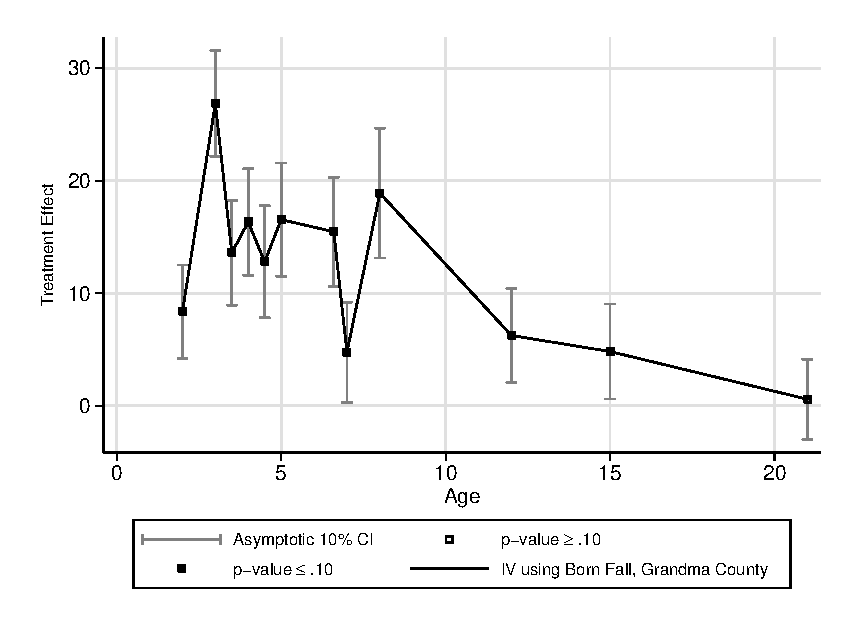
\includegraphics[width=.5\columnwidth]{output/appendixplots/main_iv_te.eps}
\floatfoot{
\footnotesize
\noindent Note: This plot presents the parameter associated to $D_i$ from an IV regression of $Y_i$ on $D_i$, $Q_i$ and $\mathbf{X_i}$, using $R_i$ and $\mathbf{Z_i}(1-R_i)$ as instruments. $Y_i$ is different IQ tests, with national standard deviation of 15 mean of 100. $\mathbf{X_i}$ includes a set of controls selected from all available baseline controls to maximize explanatory power across all outcomes tested in the paper: Male, Mother's IQ, High-Risk Index, and APGAR Score at Age 1. The confidence intervals are calculated at the 10\% significance level.}
\end{figure}

\begin{figure}[H]
		\caption{Effect of Center-based Childcare on Labor Market Outcomes, Accounting for Endogenous Take-up of Alternaive Preschool Using Instrumental Variables} \label{fig:mainiv2}
		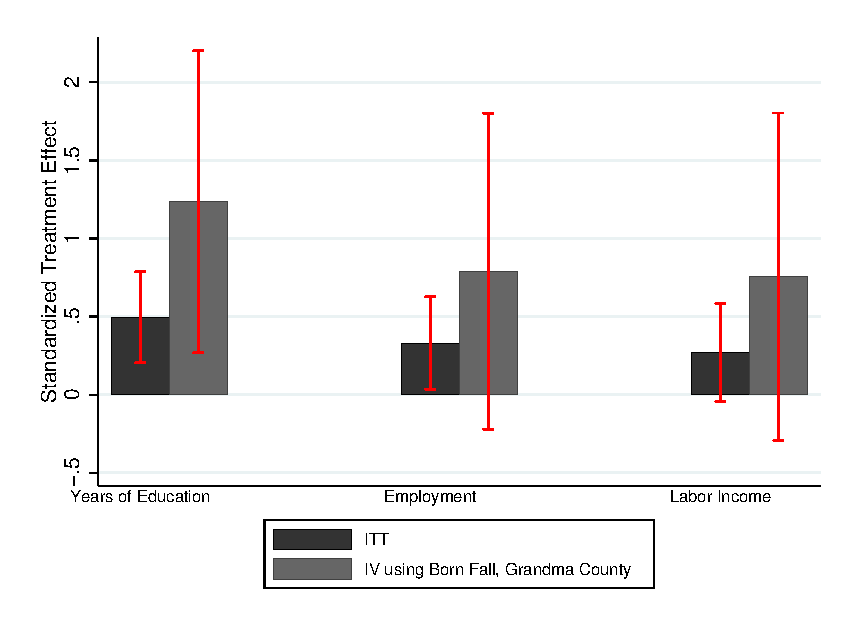
\includegraphics[width=.5\columnwidth]{output/appendixplots/main_iv_other.eps}
\floatfoot{
\footnotesize
\noindent Note: This plot presents the parameter associated to $D_i$ from an IV regression of $Y_i$ on $D_i$, $Q_i$ and $\mathbf{X_i}$, using $R_i$ and $\mathbf{Z_i}(1-R_i)$ as instruments. $Y_i$ is different relevant adult outcomes labeled in the horizontal axis. $\mathbf{X_i}$ includes a set of controls selected from all available baseline controls to maximize explanatory power across all outcomes tested in the paper: Male, Mother's IQ, High-Risk Index, and APGAR Score at Age 1. The confidence intervals are calculated at the 10\% significance level.}
\end{figure}

\subsubsection{Varying the Sets of Instruments}

\noindent Figure \ref{fig:ins_inter_Q_iv1} and Figure \ref{fig:ins_inter_Q_iv2} explores how sensitive to different sets of instruments are the instrumental variables estimates we present before. The pattern of results indicates that the method is generally robust to the three instrumental variables sets we consider. 

\begin{figure}[H]
		\caption{Effect of Center-based Childcare on IQ, Accounting for Endogenous Take-up of Alternaive Preschool Using Various Instrumental Variables} \label{fig:ins_inter_Q_iv1}
		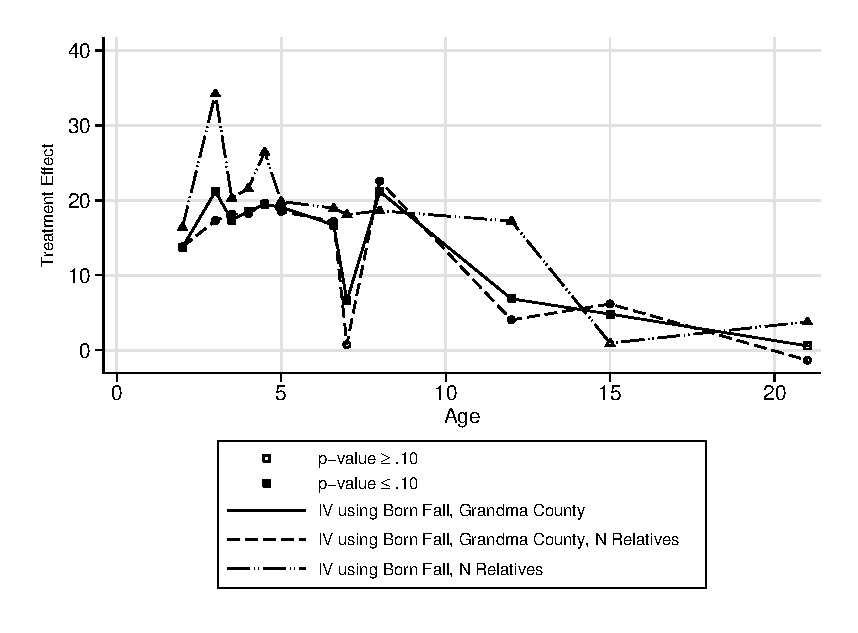
\includegraphics[width=.5\columnwidth]{output/appendixplots/ins_inter_Q_iv_te.eps}
\floatfoot{
\footnotesize
\noindent Note: This plot presents the parameter associated to $D_i$ from an IV regression of $Y_i$ on $D_i$, $Q_i$ and $\mathbf{X_i}$, using $R_i$ and $\mathbf{Z_i}(1-R_i)$ as instruments. $Y_i$ is different IQ tests, with national standard deviation of 15 mean of 100. $\mathbf{X_i}$ includes a set of controls selected from all available baseline controls to maximize explanatory power across all outcomes tested in the paper: Male, Mother's IQ, High-Risk Index, and APGAR Score at Age 1. The confidence intervals are calculated at the 10\% significance level.}
\end{figure}

\begin{figure}[H]
		\caption{Effect of Center-based Childcare on Labor Market Outcomes, Accounting for Endogenous Take-up of Alternaive Preschool Using Various Instrumental Variables} \label{fig:ins_inter_Q_iv2}
		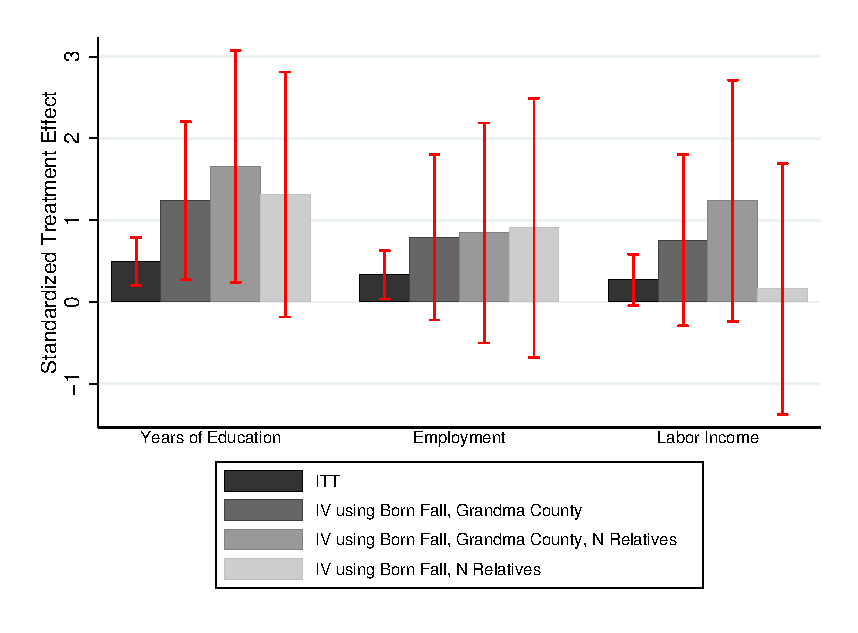
\includegraphics[width=.5\columnwidth]{output/appendixplots/ins_inter_Q_iv_other.eps}
\floatfoot{
\footnotesize
\noindent Note: This plot presents the parameter associated to $D_i$ from an IV regression of $Y_i$ on $D_i$, $Q_i$ and $\mathbf{X_i}$, using $R_i$ and $\mathbf{Z_i}(1-R_i)$ as instruments. $Y_i$ is different IQ tests, with national standard deviation of 15 mean of 100. $\mathbf{X_i}$ includes a set of controls selected from all available baseline controls to maximize explanatory power across all outcomes tested in the paper: Male, Mother's IQ, High-Risk Index, and APGAR Score at Age 1. The confidence intervals are calculated at the 10\% significance level.}
\end{figure}

\subsubsection{Varying the Specification of the Instruments}

\noindent We now present a similar exercise, exploring the sensitivity of the results to different specifications of the variables measuring take up of alternative preschools. First, Figure~ \ref{fig:nointer_Q_iv} and \ref{fig:nointer_Q_other} present the results using the set of instruments that are no interacted with ``one minis'' random assignment to center-based childcare. Figures \ref{fig:inter_Q_iv} and Figure \ref{fig:inter_Q_other} present results not only interacting the instruments but also interacting the observed characteristics we control for. In both exercises, we use $Q_i$ as the endogenous variable, along with $D_i$.\\

\noindent The results follow the same patterns as before, although there is sensitivity to not interacting the instruments. These makes economics sense because the interacted instruments better represent the economic intuition we offer before: the instruments other than $R_{i}$ are more likely to shift the decisions of the families of the control-group children, if compared to the families of the treatment-group children. 

\begin{figure}[H]
		\caption{Effect of Center-based Childcare on IQ, Accounting for Endogenous Take-up of Alternaive Preschool Using Various Instrumental Variables Specifications} \label{fig:nointer_Q_iv}
		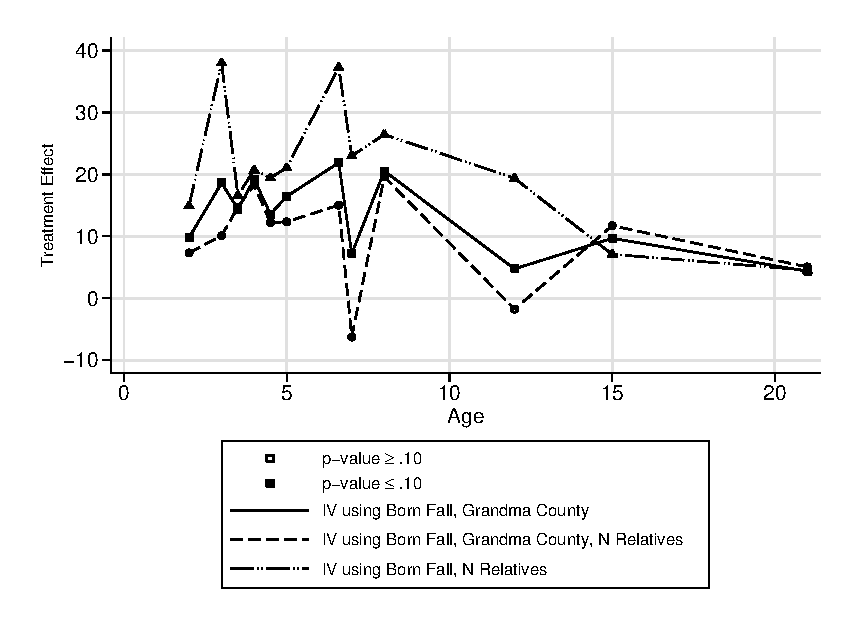
\includegraphics[width=.5\columnwidth]{output/appendixplots/nointer_Q_iv_te.eps}
\floatfoot{
\footnotesize
\noindent Note: This plot presents the parameter associated to $D_i$ from an IV regression of $Y_i$ on $D_i$, $Q_i$ and $\mathbf{X_i}$, using $R_i$ and $\mathbf{Z_i}$ as instruments. $Y_i$ is different IQ tests, with national standard deviation of 15 mean of 100. $\mathbf{X_i}$ includes a set of controls selected from all available baseline controls to maximize explanatory power across all outcomes tested in the paper: Male, Mother's IQ, High-Risk Index, and APGAR Score at Age 1. The confidence intervals are calculated at the 10\% significance level.}
\end{figure}

\begin{figure}[H]
		\caption{Effect of Center-based Childcare on Labor Market Outcomes, Accounting for Endogenous Take-up of Alternaive Preschool Using Various Instrumental Variables Specifications} \label{fig:nointer_Q_other}
		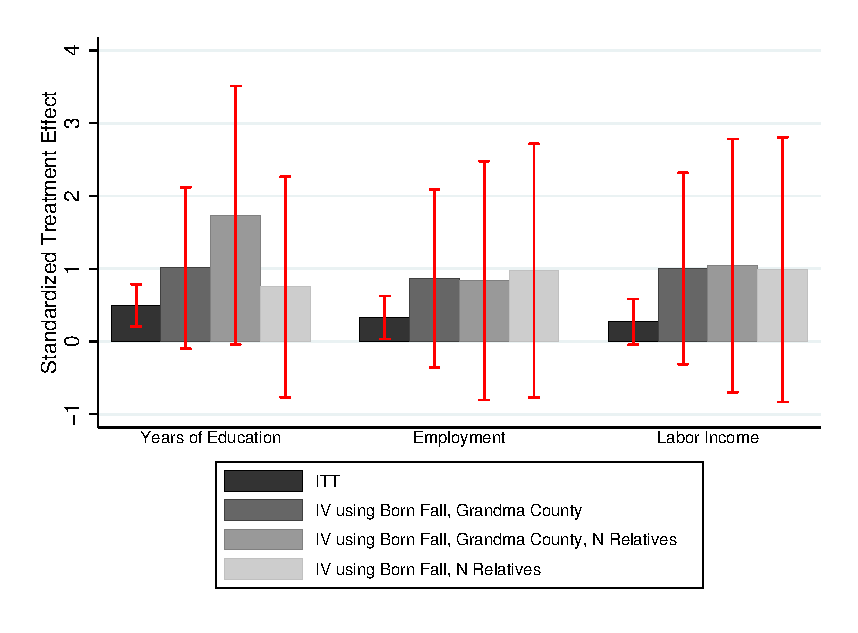
\includegraphics[width=.5\columnwidth]{output/appendixplots/nointer_Q_iv_other.eps}
\floatfoot{
\footnotesize
\noindent Note: This plot presents the parameter associated to $D_i$ from an IV regression of $Y_i$ on $D_i$, $Q_i$ and $\mathbf{X_i}$, using $R_i$ and $\mathbf{Z_i}$ as instruments. $Y_i$ is different IQ tests, with national standard deviation of 15 mean of 100. $\mathbf{X_i}$ includes a set of controls selected from all available baseline controls to maximize explanatory power across all outcomes tested in the paper: Male, Mother's IQ, High-Risk Index, and APGAR Score at Age 1. The confidence intervals are calculated at the 10\% significance level.}
\end{figure}

\begin{figure}[H]
		\caption{Effect of Center-based Childcare on IQ, Accounting for Endogenous Take-up of Alternaive Preschool Using Various Instrumental Variables Specifications} \label{fig:inter_Q_iv}
		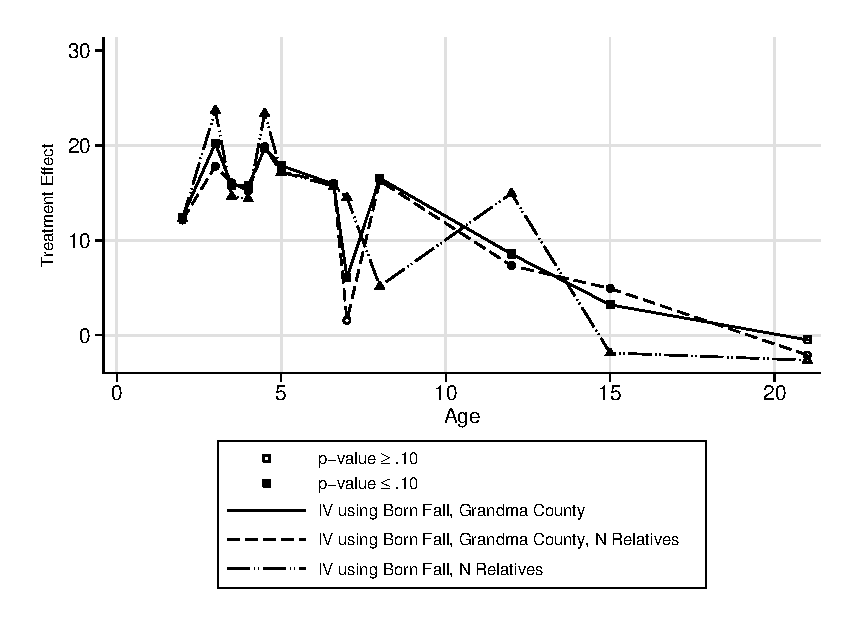
\includegraphics[width=.5\columnwidth]{output/appendixplots/inter_Q_iv_te.eps}
\floatfoot{
\footnotesize
\noindent Note: This plot presents the parameter associated to $D_i$ from an IV regression of $Y_i$ on $D_i$, $Q_i$ and $\mathbf{X_i}$, using $R_i$, $\mathbf{X_i}(1 - R_i)$ and $\mathbf{Z_i}(1 - R_i)$ as instruments. $Y_i$ is different IQ tests, with national standard deviation of 15 mean of 100. $\mathbf{X_i}$ includes a set of controls selected from all available baseline controls to maximize explanatory power across all outcomes tested in the paper: Male, Mother's IQ, High-Risk Index, and APGAR Score at Age 1. The confidence intervals are calculated at the 10\% significance level.}
\end{figure}

\begin{figure}[H]
		\caption{Effect of Center-based Childcare on Labor Market Outcomes, Accounting for Endogenous Take-up of Alternaive Preschool Using Various Instrumental Variables Specifications} \label{fig:inter_Q_other}
		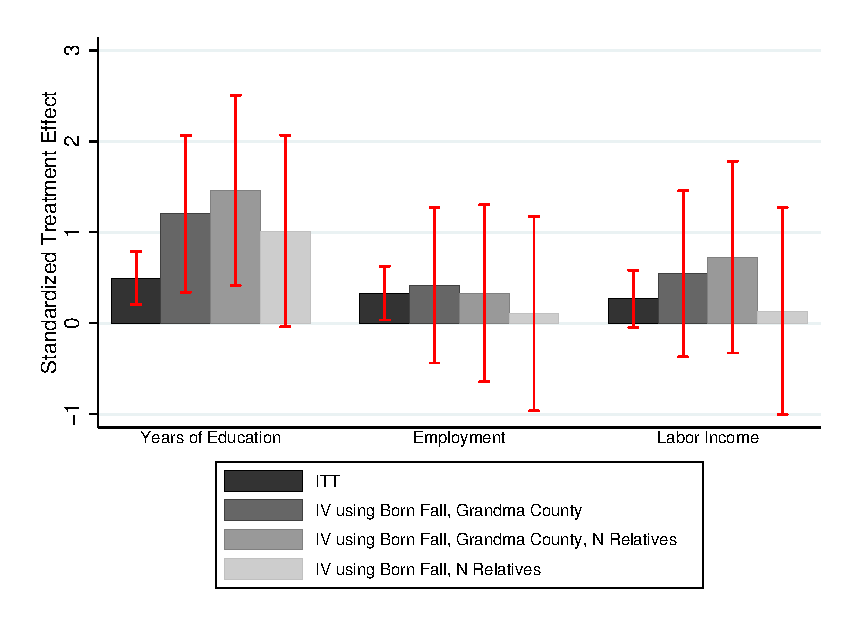
\includegraphics[width=.5\columnwidth]{output/appendixplots/inter_Q_iv_other.eps}
\floatfoot{
\footnotesize
\noindent Note: This plot presents the parameter associated to $D_i$ from an IV regression of $Y_i$ on $D_i$, $Q_i$ and $\mathbf{X_i}$, using $R_i$, $\mathbf{X_i}(1 - R_i)$ and $\mathbf{Z_i}(1 - R_i$) as instruments. $Y_i$ is different IQ tests, with national standard deviation of 15 mean of 100. $\mathbf{X_i}$ includes a set of controls selected from all available baseline controls to maximize explanatory power across all outcomes tested in the paper: Male, Mother's IQ, High-Risk Index, and APGAR Score at Age 1. The confidence intervals are calculated at the 10\% significance level.}
\end{figure}

\subsubsection{Varying the Parameterization of Alternative Preschool Take-up}

\noindent Now, we explore the sensitivity to the specification of $Q_{i}$ in \eqref{eq:ivnot}. We consider two alternatives. First, specifying it as an indicator for preschool alternatives take-up, $P_{i}$ (Figure~\ref{fig:ins_inter_P_iv} and Figure~\ref{fig:ins_inter_P_other}). Second, taking the $\log$ of $Q_{i}$ (Figure~\ref{fig:ins_inter_LogQ_iv} and Figure~\ref{fig:ins_inter_LogQ_other}).

\begin{figure}[H]
		\caption{Effect of Center-based Childcare on IQ, Accounting for an Endogenous Indicator of Take-up of Alternaive Preschool} \label{fig:ins_inter_P_iv}
		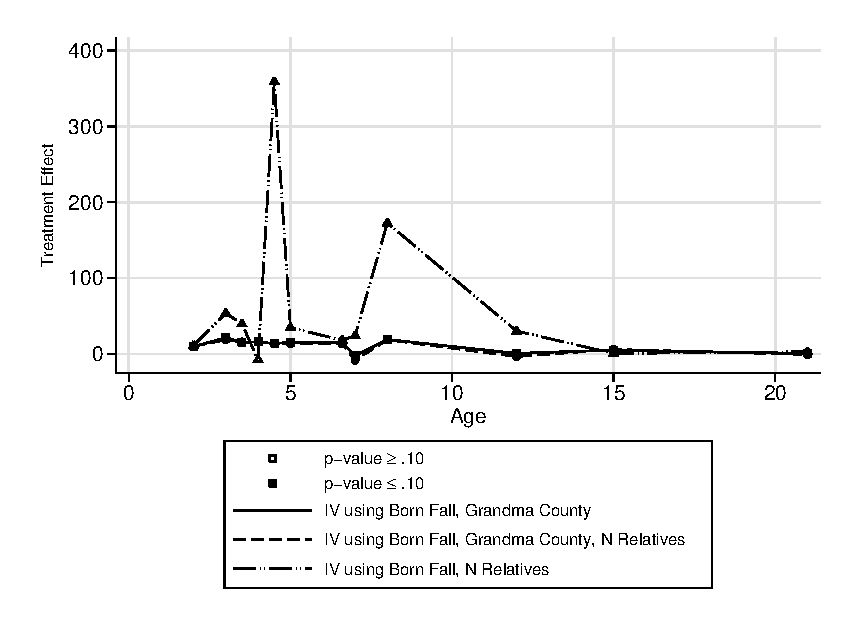
\includegraphics[width=.5\columnwidth]{output/appendixplots/ins_inter_P_iv_te.eps}
\floatfoot{
\footnotesize
\noindent Note: This plot presents the parameter associated to $D_i$ from an IV regression of $Y_i$ on $D_i$, $P_i$ and $\mathbf{X_i}$, using $R_i$, $\mathbf{Z_i}(1 - R_i)$ as instruments. $Y_i$ is different IQ tests, with national standard deviation of 15 mean of 100. $\mathbf{X_i}$ includes a set of controls selected from all available baseline controls to maximize explanatory power across all outcomes tested in the paper: Male, Mother's IQ, High-Risk Index, and APGAR Score at Age 1. The confidence intervals are calculated at the 10\% significance level.}
\end{figure}

\begin{figure}[H]
		\caption{Effect of Center-based Childcare on Labor Market Outcomes, Accounting for an Endogenous Indicator of Take-up of Alternaive Preschool} \label{fig:ins_inter_P_other}
		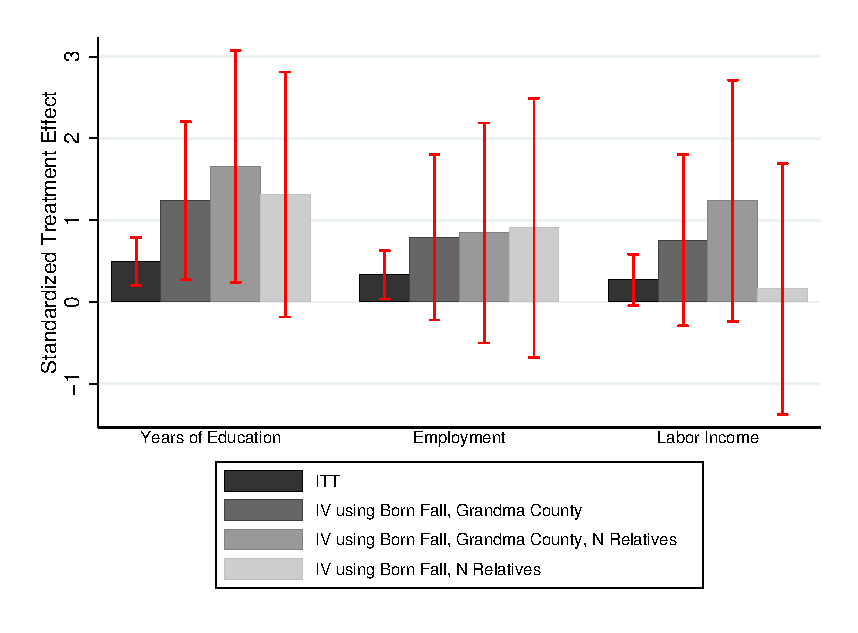
\includegraphics[width=.5\columnwidth]{output/appendixplots/ins_inter_P_iv_other.eps}
\floatfoot{
\footnotesize
\noindent Note: This plot presents the parameter associated to $D_i$ from an IV regression of $Y_i$ on $D_i$, $P_i$ and $\mathbf{X_i}$, using $R_i$, $\mathbf{Z_i}(1 - R_i$) as instruments. $Y_i$ is different IQ tests, with national standard deviation of 15 mean of 100. $\mathbf{X_i}$ includes a set of controls selected from all available baseline controls to maximize explanatory power across all outcomes tested in the paper: Male, Mother's IQ, High-Risk Index, and APGAR Score at Age 1. The confidence intervals are calculated at the 10\% significance level.}
\end{figure}

\begin{figure}[H]
		\caption{Effect of Center-based Childcare on IQ, Accounting (log) Months Endogenous of Take-up of Alternaive Preschool} \label{fig:ins_inter_LogQ_iv}
		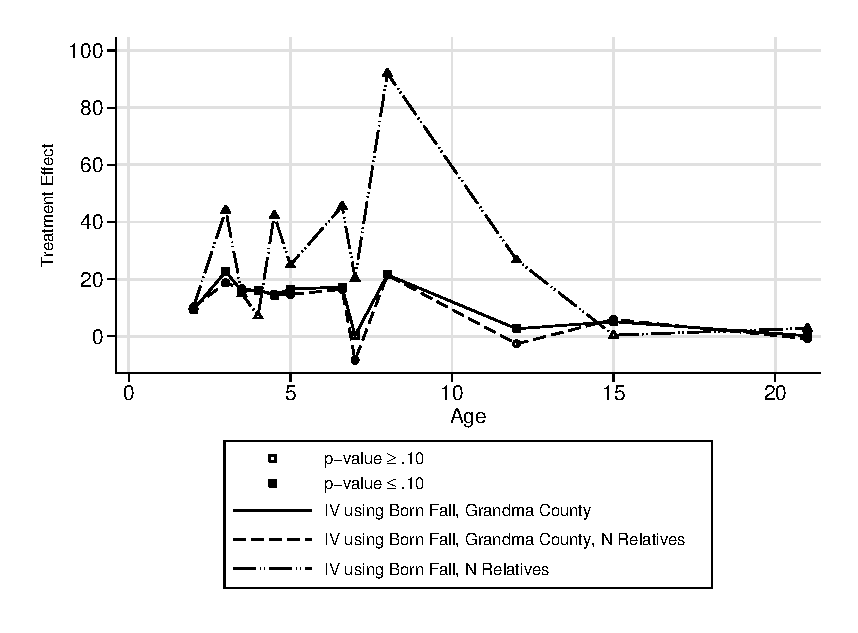
\includegraphics[width=.5\columnwidth]{output/appendixplots/ins_inter_logQ_iv_te.eps}
\floatfoot{
\footnotesize
\noindent Note: This plot presents the parameter associated to $D_i$ from an IV regression of $Y_i$ on $D_i$, $\log Q_i$ and $\mathbf{X_i}$, using $R_i$, $\mathbf{Z_i}(1 - R_i)$ as instruments. $Y_i$ is different IQ tests, with national standard deviation of 15 mean of 100. $\mathbf{X_i}$ includes a set of controls selected from all available baseline controls to maximize explanatory power across all outcomes tested in the paper: Male, Mother's IQ, High-Risk Index, and APGAR Score at Age 1. The confidence intervals are calculated at the 10\% significance level.}
\end{figure}

\begin{figure}[H]
		\caption{Effect of Center-based Childcare on Labor Market Outcomes, Accounting (log) Months Endogenous of Take-up of Alternaive Preschool} \label{fig:ins_inter_LogQ_other}
		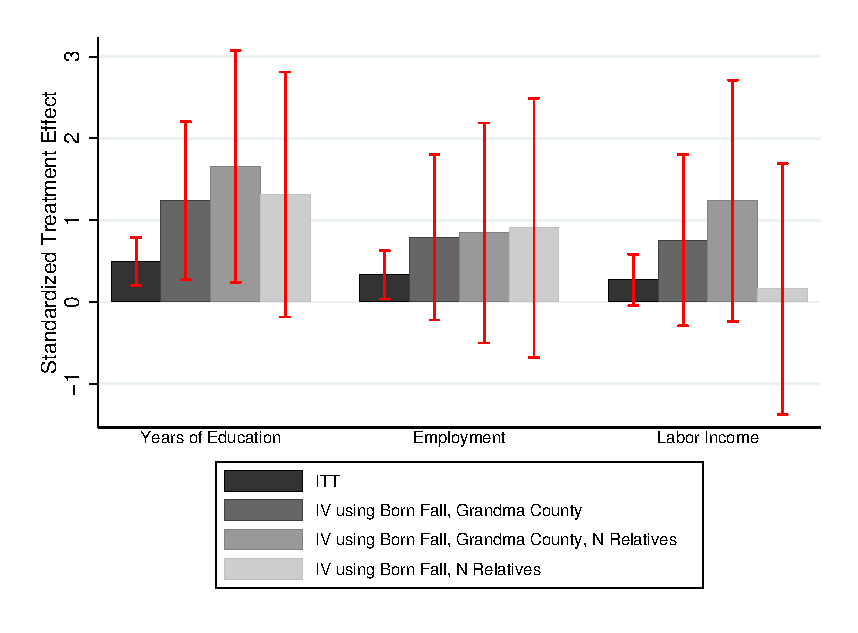
\includegraphics[width=.5\columnwidth]{output/appendixplots/ins_inter_logQ_iv_other.eps}
\floatfoot{
\footnotesize
\noindent Note: This plot presents the parameter associated to $D_i$ from an IV regression of $Y_i$ on $D_i$, $\log Q_i$ and $\mathbf{X_i}$, using $R_i$, $\mathbf{Z_i}(1 - R_i$) as instruments. $Y_i$ is different IQ tests, with national standard deviation of 15 mean of 100. $\mathbf{X_i}$ includes a set of controls selected from all available baseline controls to maximize explanatory power across all outcomes tested in the paper: Male, Mother's IQ, High-Risk Index, and APGAR Score at Age 1. The confidence intervals are calculated at the 10\% significance level.}
\end{figure}


\subsection{Control Functions}

\noindent We now consider a control function approach. In this, the objective is also to simultaneously account for take-up of center-based childcare and preschool alternatives. 

\subsubsection{Setup}

\noindent The method we propose is an application of of the selection correction in \citet{Heckman_1979_Econometrica}. We model the selection into both endogenous variables of interest, center-based childcare and preschool alternatives. The method involves three equations: (i) the outcome equation; (ii) the probability of participating in center-based childcare; (iii) a linear equation describing the number of months enrolled in preschool alternatives.\\

\noindent Let $Y^{0}_{i}$ be the counterfactual outcome of child $i$ when not participating of center-based childcare. Similarly, let $Y^{1}_{i}$ be her potential outcome if she participates. We model the outcome as: 
 
\begin{eqnarray}
Y_{i}^1 &=& \alpha^1+\mathbf{X}_{i} \mathbf{\beta}                 +\varepsilon_i^1 \nonumber  \\
Y_{i}^0 &=& \alpha^0+\mathbf{X}_{i} \mathbf{\beta} + \alpha^Q Q_i+\varepsilon_i^0.  \label{eq:potout}
\end{eqnarray}

\noindent The equation describing participation in center-based childcare is: 

\begin{equation}
D_{i} = \left\{
        \begin{array}{ll}
        	0 &\text{if } D_{i}^* \leq  0 \\
            1 &\text{if } D_{i}^* > 0, \label{eq:sel1}
        \end{array}
    \right. 
\end{equation}

\noindent where we interpret $D_{i}^*$ as a latent continuous variable representing the household's interest in sending the child to preschool. We write

\begin{equation}
D^{*}_i = \mathbf{W}_i \gamma^{D} + \varepsilon^{D}_i, \label{eq:probitD}
\end{equation}

\noindent where $\mathbf{W}_i$ is a vector that includes $\mathbf{X}_i$ and can include variables that shift the decision to enroll children into ABC/CARE without shifting the counterfactual outcome of interest, $Y^{d}_{i}$. The most important of those variables is $R_i$, randomization to treatment.\\

\noindent We write the selection equation into months of preschool as a linear equation with fixed coefficients, assuming homogeneous treatment effects:

\begin{equation}
Q_i = \mathbf{W}_i \gamma^{Q} + \varepsilon^{Q}_i, \label{eq:selq}
\end{equation}

\noindent In general, the unobserved variables in each of these equations are correlated. We assume that they are distributed as follows: 

\begin{equation}
        \left[ \begin{array}{l}
        	 \varepsilon_{i}^1 \\
            \varepsilon_{i}^0 \\
            \varepsilon_{i}^D
        \end{array} \right]  \sim \mathcal{N} \left[ \left( \begin{array}{l}
        	 0 \\
           0 \\ 
           0
        \end{array} \ \right), 
                \left( \begin{array}{llll}
        	 \sigma_{1}^2 & \sigma_{1,0} & \sigma_{1,D}   \\
             \sigma_{1,0} & \sigma_{0}^2 & \sigma_{0,D}   \\
             \sigma_{1,D} & \sigma_{0,D} & 1 
        \end{array} \right) \right],  \label{eq:udist}
\end{equation}

\noindent where we normalize $\var \left( \varepsilon^D_i \right) =1$.\\

\noindent Further, we assume that 
\begin{equation}
\mathbb{E}\left[\varepsilon_i^0|D_i=0,\mathbf{W}_i,\varepsilon^{Q}_i,Q_i=q\right]=\sigma^{0Q}\varepsilon^{Q}_i+\mathbb{E}\left[\varepsilon_i^0|D_i=0,\mathbf{W}_i\right].
\label{eq:E[epsilon0]}
\end{equation}

\subsubsection{Identification}

\noindent To identify the parameters of interest, we follow these steps. First, we estimate the parameters characterizing the decision to enroll the child in center-based childcare. We exploit the assumption that $\varepsilon_{i}^D \sim \mathcal{N} \left( 0, 1 \right)$ in \eqref{eq:udist} and estimate the parameters in equation \eqref{eq:probitD} using a probit model.\\

\noindent Second, we approximate the unobserved term relevant to the choice of $Q_{i}$. We the coefficients in \eqref{eq:selq} to obtain an estimate for$\varepsilon^{Q}_i$. By linearly conditioning on this term, we account for the correlation between the error term in the decision for $Q_{i}$ and the error term in the outcome equations, $\varepsilon_i^0$.\\

\noindent Third, we estimate the coefficients in the outcome equation using the proxies for the unobserved components. We rewrite \eqref{eq:potout} using conditional expectations:

\begin{eqnarray}
\mathbb{E}\left[Y_i^1|D_i=1,\mathbf{W}_i\right]                         &=& \alpha^1+\mathbf{X}_i\mathbf{\beta}              +\mathbb{E}\left[\varepsilon_i^1|D_i=1,\mathbf{W}_i      \right] \nonumber \\
\mathbb{E}\left[Y_i^0|D_i=0,\mathbf{W}_i,\varepsilon^{Q}_i,Q_i=q\right] &=& \alpha^0+\mathbf{X}_i\mathbf{\beta} +\alpha^Q q \label{eq:condout} \\ \nonumber && \quad + \mathbb{E}\left[\varepsilon_i^0|D_i=0,\mathbf{W}_i,\varepsilon^{Q}_i,Q_i=q\right].
\end{eqnarray}

\noindent Once we condition on the proxy for $\varepsilon^{Q}_i$, the error term in the outcome equations only depends on the selection into center-based childcare. The conditional error terms in equation \eqref{eq:condout} can be specified as control functions.\\ 

\noindent For children enrolled in treatment, the control function is: 
\begin{equation}
\mathbb{E} \left[\varepsilon_i^1|D_i=1,\mathbf{W}_i \right]=\sigma_1\frac{\phi \left( \mathbf{W}_i \gamma^D \right) }{ \Phi \left( \mathbf{W}_i \gamma^D \right) }. \label{eq:contam}
\end{equation}

\noindent For children not enrolled in the treatment, the control function is:
\begin{equation}
\mathbb{E} \left[\varepsilon_i^0|D_i=0,\mathbf{W}_i,\varepsilon^{Q}_i,Q_i=q\right]= \sigma^{0Q}\varepsilon^{Q}_i - \sigma_0 \frac{\phi\left(\mathbf{W}_i\gamma^D\right)}{\Phi\left( - \mathbf{W}_{i} \gamma^D \right) }. \label{eq:home}
\end{equation}

\subsection{Estimates}

\noindent The methodology we propose allows to recover consistent estimates of the parameters in \eqref{eq:potout} through a linear regression by including the control functions. The effect of center-based childcare is the difference of the difference in the intercepts in the two outcome equations.\\

\noindent The charts below presents the estimates for the parameter associated to $D_i$. That is, the effect of participating of center-based childcare, relative to a counterfactual of receiving no preschool alternative. As before, we present results for a set of IQ tests and for a set of relevant adult outcomes. The results are not compelling, as they present irregularities over the life-cycle that differs from the rest of results we present in the main paper and throughout this appendix. 

\begin{figure}[H]
		\caption{Effect of Center-based Childcare on Labor Market Outcomes, Accounting (log) Months Endogenous of Take-up of Alternaive Preschool} \label{output/appendixplots/Q_cf_te.eps}
		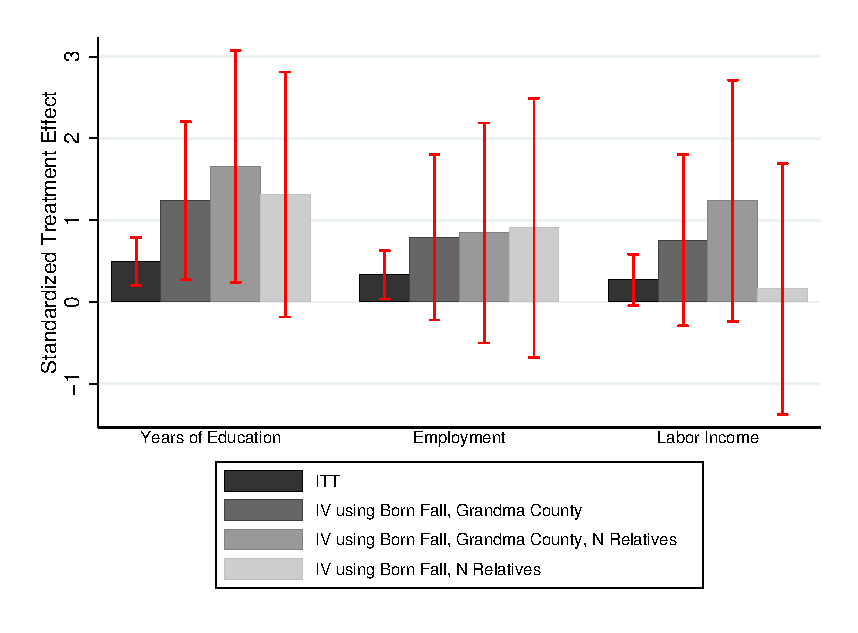
\includegraphics[width=.5\columnwidth]{output/appendixplots/ins_inter_logQ_iv_other.eps}
\floatfoot{
\footnotesize
\noindent Note: This plot presents the parameter associated to $D_i$ estimated using Control Functions as described in the text. $Y_i$ is different IQ tests with national standard deviation of 15 and mean of 100.  $D_i=1$ for children that participate in ABC or CARE center-based treatment, and $D_i=0$ for children in the control or home visits groups. $Q_i$ is the number of months attending preschool. It is coded as zero for children participating in ABC/CARE. $\mathbf{X_i}$ includes a set of controls selected from all available baseline controls to maximize explanatory power across all outcomes tested in the paper: Male, Mother's IQ, High-Risk Index, and APGAR Score at Age 1.}
\end{figure}

\setcounter{figure}{0}  \renewcommand{\thefigure}{D.\arabic{figure}}
\setcounter{table}{0}   \renewcommand{\thetable}{D.\arabic{table}}
\section{Assessing Common Critiques to ABC} \label{appendix:assessingcc}

\noindent This section of the appendix assesses some of the critiques to ABC, which could apply to CARE as well. The critiques focus on the first phase of the program, to which we refer simply as ABC in this section of the appendix.\\

\noindent The first critique we assess is that of \citet{Spitz_1992_ABC-Retardation}. The author asks if ABC prevented socio-cultural mental retardation. He focuses on different measures of cognition, and generically calls them IQ. His main focus is on the raw mean difference between the treatment and the control groups in the Bayley Mental Development Index (MDI) at age 1.\footnote{The Bayley Mental Development Index is a standard measure of cognition at taken between ages 0 and 2 \citep{Childrens-Health_2016_Bayley-Scales}.} He finds a noticeable disparity in the mean difference between cohorts 1 and 2 and cohorts 3 and 4, as early as six months after the treatment began. As \citet{Spitz_1992_ABC-Retardation} argues, this difference is conspicuous and we display it in Table~\ref{table:cohorts}. Importantly, the author fails to note that the mean differences have noticeably high standard errors.

\begin{table}[H] 
\begin{threeparttable}
\caption{Treatment - Control Mean Difference by Cohort, ABC}
\label{table:cohorts}
\centering 
\begin{tabular}{lcc} \toprule
 & (1) & (2) \\
 & Bayley MDI, 12 Months & Bayley MDI, 24 Months \\ \midrule
 &  &  \\\
Cohort 1 & 4.841 & -2.901 \\
 & (6.013) & (5.926) \\
Cohort 2 & 0.071 & 1.882 \\
 & (6.013) & (5.830) \\
Cohort 3 & 9.143 & 10.038 \\
 & (5.801) & (5.926) \\
Cohort 4 & 7.829 & 13.713 \\
 & (5.801) & (5.830) \\ \\ \midrule
Observations & 112 & 110 \\
$R^2$ & 0.055 & 0.110 \\ \bottomrule
 \end{tabular}
\begin{tablenotes}
\footnotesize
\item Note: This table displays the mean difference between the treatment and control groups in two measures of the Bayley Mental Development Index, for ABC. Homoskedastic, asymptotic standard errors are in parentheses.
\end{tablenotes}
\end{threeparttable}
\end{table}

\noindent \citet{Spitz_1992_ABC-Retardation} states that: ``an essential question is whether the differences at 6 months of age were due to the intervention or were preexisting'' \citep[][p. 230]{Spitz_1992_ABC-Retardation}. \citet{Spitz_1992_ABC-Retardation} proceeds with speculative exercises that lead him to state that it is questionable to conclude that the mean difference between the treatment and control groups as early as age six months is a consequence of the treatment.\footnote{The exact quote is: ``Even if the differences between experimental and control groups at 6 months of age were a consequence of the first few months of intervention, which is questionable, the negligible additional effects after age 4.5 more years in the program should at least make one cautious about this kind of intervention's potential [\ldots]'' \citep[][p. 235]{Spitz_1992_ABC-Retardation}. We asses the former point before getting to the latter.}\\

\noindent His argument stem from not receiving information on the maternal characteristics which he considers fundamental for his analysis to comparing test scores over the years.\footnote{He does not note that tests scores \textit{do not have a well-defined scale} and are hard to compare.}\\ 

\noindent We make three annotations with respect to the comments in \citet{Spitz_1992_ABC-Retardation}.\\ 

\noindent \textbf{1. In neither cohorts of ABC do mothers significantly differ in observed characteristics between the treatment and the control groups.} When jointly testing the hypothesis of differences in a battery of observed characteristics, we fail to reject any difference between the families of these children (see Table~\ref{tab:baseline_coh1} to Table~\ref{tab:baseline_coh4}). Even when the point estimates present some differences, they are minimal. For example, treatment-group mothers differ from control-group mothers, on average, by having one more point in the IQ score, which has a population standard deviation of 15.\\

\noindent \textbf{2. Other early childhood education programs have generated gains in cognition very early in life, as soon as a year after the program begins.} A more recent program, the Infant Health and Development Program (IHDP), treated children from ages 0 to 3. \citet{Gross_Spiker_etal_1997_BOOKHelpinglowbirth} thoroughly describe this program. A lot of its elements were based on ABC and CARE. The program offered an average of eight hours a week of center-based childcare from ages 1 to 3, weekly home visits from ages 0 to 1, and bi-monthly home visits from ages 1 to 3. Measures on the Bayley MDI at 12 and 24 months are available. The most intensive part of the treatment, center-based childcare, began at age 12 months in IHDP while it began at birth in ABC. As in ABC, after a few months of center-based childcare, the effects on cognition were substantial in IHDP.

\begin{table}[H] 
\begin{threeparttable}
\caption{Treatment - Control Mean Difference, IHDP}
\label{table:ihdp}
\centering 
\begin{tabular}{lcc} \hline \hline
 & (1) & (2) \\
 & Bayley MDI, 12 Months & Bayley MDI, 24 Months \\ \hline
 &  &  \\\
Mean Treatment - Mean Control & 0.142 & 9.958 \\
 & (0.968) & (1.498) \\
 &  &  \\ \hline
Observations & 893 & 910 \\
$R^2$ & 0.000 & 0.067 \\ \hline \hline  
\end{tabular}
\begin{tablenotes}
\footnotesize
\item Note: This table displays the mean difference between the treatment and control groups in two measures of the Bayley Mental Development Index, for the Infant Health and Development Program using the principal analysis sample. Robust standard errors clustered by state and an indicator of weight below 2,000 grams in parentheses.
\end{tablenotes}
\end{threeparttable}
\end{table}


\noindent \textbf{3. The effects on cognition are sustained throughout childhood and up to age 21 even when partialing out the Bayley MDI at ages 12 and 24 months.} When partialing out in a linear regression the score in the Bayley MDI tests both at twelve and twenty-four months of age, the treatment effects on cognition, measured by the mean difference between the treatment and the control groups in different IQ test scores, are still significant and are sustained up to age 21 (see Figure~\ref{fig:treatiqsabc}).

\begin{figure}[H]
		\caption{Treatment Effects on IQ, ABC} \label{fig:treatiqsabc}
		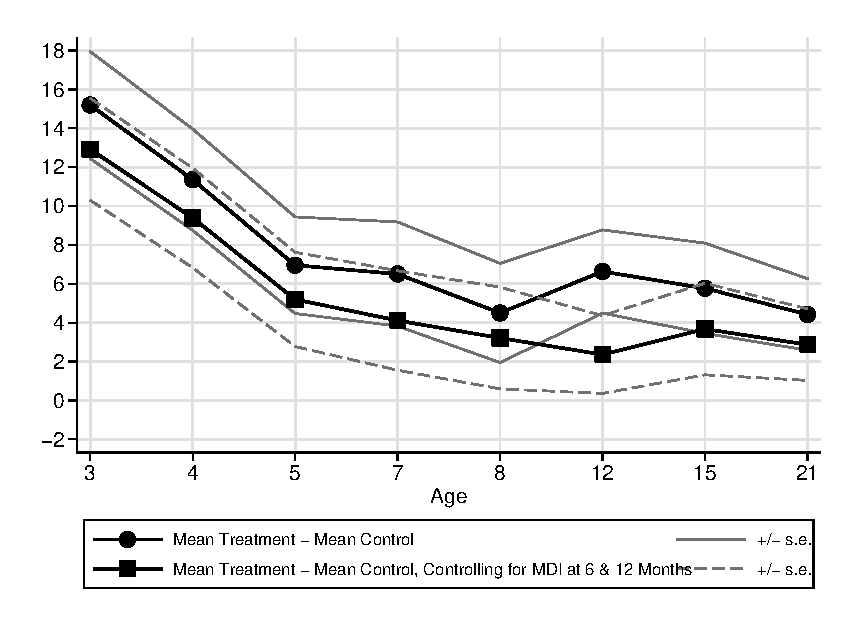
\includegraphics[width=.9\columnwidth]{output/abc_mdifixing_2.eps}
\floatfoot{
\footnotesize
\noindent Note: This figure displays the mean difference between the treatment and the control groups in IQ at different ages, pooling males and females. The circled line represents the raw difference. The squared line represents the difference when linearly controlling for the Bayley Mental Development Index at 6 and 12 months.}
\end{figure}

\noindent The author raises an additional concern. He states that even if the early-life effects on the Bayley MDI were true, the effects were not long-lasting. When doing so, he exclusively refers to the effects the program had on cognition. As we vastly document throughout the main paper, however, ABC had effects on a wide set of life-cycle outcomes, which perhaps are more important than the effects on cognition if measured by the economic gains they generate. Examples include: employment at age 30 for males, high-school graduation for females, and a variety of health measures at age 34 for males. We document these effects in the main paper.\\

\noindent This critique relates to a second critique that has been made to ABC.\footnote{See, for example, \citet{Besharov-etal_2011_ABCProject}.} Mostly based on the fade-out of the effects on cognition and on results on age-21 outcomes, some studies claim that ABC had no sustained long-term effects. In addition to the evidence we cite above, it is important to add the following.\\

\noindent  \textbf{4. The treatment effects of ABC differed by gender.} For example, we find substantial effects on employment for males and high-school graduation for females. This does not mean that the program did not work. It means that market conditions could affect the way in which the participants of the program could have benefited from its effects.\\

\begin{sidewaystable}[H] 
\begin{threeparttable}
\caption{Randomization Compromises, ABC}
\label{table:abccompromises}
\centering
\footnotesize
\begin{tabular}{ccccc} \toprule
Child ID & Initial Assignment & Compromise Description & Data Availability & Methodology Assumption \\ \\ \midrule
Case A & Treatment & Left the study & None & Missing at random \\
Case B & Treatment & Left the study & None & Missing at random \\
Case C & Treatment & Left the study & None & Missing at random \\
Case D & Treatment & Left the study & None & Missing at random \\ \midrule
.x    & Control  & Died (age 0), heart disease & Baseline; before dead & Attrition after death \\
914 & Control  & Died (age 0), heart disease & Baseline; before dead & Attrition after death \\
74 & Treatment & Died (age 0), SIDS & Baseline; before dead & Attrition after death \\
99 & Treatment  & Died (age 4), pedestrian accident & Baseline; before dead & Attrition after death \\ \midrule
900 & Treatment  & Non-compliance  & Baseline; before age 8 & Attrition after age 8  \\
912 & Treatment  & Non-compliance  & Baseline; before age 8 & Attrition after age 8  \\
922 & Treatment  & Non-compliance  & Baseline; before age 8 & Attrition after age 8  \\ \midrule
78  & Control        & Crossover from control to treatment & Baseline; before age 8 & Attrition after age 8  \\ \midrule
85 & Treatment   & 3 months of treatment &  Baseline; after age 2 & Same as treatment group  \\  
103 & Treatment &10 months of treatment &  Baseline; after age 2 & Same as treatment group  \\
108 & Treatment & 6 months of treatment &  Baseline; after age 2 & Same as treatment group  \\ 
123 & Treatment & 9 months of treatment &  Baseline; after age 2 & Same as treatment group  \\  \midrule
906 & Control  & Left study at 54 months & Baseline; before 54 months & Attrition after 54 months \\ \midrule
95   & Treatment       & Developmentally delayed at 6 months & No data after diagnosis & Dropped (non-eligible) \\ 
124 & Treatment       & Developmentally delayed at 36 months & No data after diagnosis & Dropped (non-eligible) \\ \midrule
 82 & Control       & Crossover from control to treatment & Baseline, before age 8 & Dropped (non-eligible)  \\ 
 119 & Control       & Crossover from control to treatment & Baseline, before age 8 & Dropped (non-eligible)  \\ \bottomrule
\end{tabular}
\begin{tablenotes}
\item Note: This table describes the various randomization compromises in ABC. For each child, we display: the ID assigned by the program staff, the nature of the compromise, the data available, and the methodological assumption when accounting for non-compliance and program attrition. 
\end{tablenotes}
\end{threeparttable}
\end{sidewaystable}

\noindent The third and last critique we assess is that of compromised randomization.\footnote{See for example \citet{Baumeister-Bacharach_2000_Early-Generic} and the multiple studies cited there.} The main critique to the program in this respect is that seven children in the treatment group did not comply to their initial assignment and one child switched from control to treatment status. This critique refers to the children labeled with the following IDs by the program: N/A Case A, N/A Case B, N/A Case C, N/A Case D, 900, 912, 922, and 78 (see Table~\ref{table:abccompromises}, which we reproduce from the main paper). Although we document more cases of compromised randomization, we start by assessing these eight cases.\footnote{Our main methodology assesses all the cases except the children for whom we do not have data at all (Case A, N/A Case B, N/A Case C, N/A Case D). We are not able to account for them because our method is based on observing at least some baseline characteristics. See Section~\ref{section:methodology} in the main paper for more details.}\\

\noindent First, we propose a method to assess the non-compliance of children 900, 912, 922, and 78, for whom we have data available from ages 0 to 8. This allows for the possibility to adjust the mean difference between the treatment and the control groups, using a standard Bloom estimator \citep{Bloom_1984_ER}. This estimator accounts for compliance, by weighting the mean difference by a measure of the probability of compliance. It takes the following form: 

\begin{equation}
\Delta^{\textbf{Bloom}} = \frac{\mathbb{E} \left[ Y | R = 1 \right] - \mathbb{E} \left[ Y | R = 0 \right] }{\mathbb{E} \left[ D = 1 | R = 1 \right] - \mathbb{E} \left[ D = 0 | R = 0 \right]}, 
\end{equation}

\noindent where $R$ indicates randomization into treatment, $D$ indicates treatment take-up, and $Y$ is an outcome of interest.\\

\noindent This estimator has gained attention as it coincides with the instrumental variables estimator of the parameter in linear regression of an outcome on a single explanatory variable, e.g. treatment take-up. As \citet{Angrist_Imbens_ea_1996_JASA} show, under certain assumptions it can be interpreted as the average treatment effect for those individuals induced to take up treatment by the instrument. This interpretation has various weaknesses \citep{Heckman_Urzua_etal_2006_REStat,Heckman_Urzua_2010_JoE}.\\

\noindent To compare the mean difference and the Bloom estimator we consider two measures of cognition, which are commonly used when evaluating ABC and are available for children 900, 912, 922, and 78: the Stanford Binet IQ test at age 3 and the Wechsler Preschool and Primary Scale of Intelligence at age 5. Table~\ref{table:nc1} presents the results and shows that the differences are minimal. \textbf{5. Adjusting for the non-compliance of children 900, 912, 922, and 78 makes little difference} when assessing outcomes for which we observe these children. 

\begin{table}[H] 
\begin{threeparttable}
\caption{Assessing Non-compliance in ABC, Exercise 1}
\label{table:nc1}
\centering 
\begin{tabular}{ccccc} \toprule
 & (1) & (2) & (3) & (4) \\
 & IQ, Age 3 & IQ, Age 3  & IQ, Age 5 & IQ, Age 5 \\ \midrule
 &  &  & & \\\
Treatment - Control Mean Difference & 14.970 &  & 6.398 &  \\
 & (2.794) &  & (2.494) &  \\
Bloom &  & 16.245 &  & 6.943 \\
 &  & (2.877) &  & (2.643) \\ \midrule
Observations & 100 & 100 & 100 & 100  \\
 $R^2$ & 0.227 & 0.289 & 0.063 & 0.088 \\ \bottomrule
 \end{tabular}
\begin{tablenotes}
\footnotesize
\item Note: This table displays the mean difference between the treatment and control groups and the same difference adjusted for non-compliance (Bloom estimator) in two measures of IQ, the Stanford-Binet IQ Score at age 3 and the Wechsler Preschool and Primary Scale of Intelligence at age 5. Homoskedastic, asymptotic standard errors are in parentheses.
\end{tablenotes}
\end{threeparttable}
\end{table}


\noindent Second, we propose a method to account for non-compliance of the children N/A Case A, N/A Case B, N/A Case C, N/A Case D. For them, we have no data at all. We reproduce the estimates in Table~\ref{table:nc2}, assigning to each of these four children the worst score across all the children in the treatment group, for each of the tests we consider---the worst score was 71 for both the age-3 and the age-5 measures. \textbf{6. Even when assigning the worst score to the children who did not comply to treatment and for whom no data is available, the mean difference between treatment and control is sizable and not significantly different from the baseline cases where we do not adjust for non-compliance cases} (columns (1) and (3) in Table~\ref{table:nc1}).

\documentclass[]{article}
\setlength{\pdfpagewidth}{8.5in} \setlength{\pdfpageheight}{11in}
\begin{document}
\begin{tabular}{lcccc} \hline
 & (1) & (2) & (3) & (4) \\
 & iq3y\_itt & iq3y\_iv & iq5y\_itt & iq5y\_iv \\
VARIABLES & IQ at age 3y months & IQ at age 3y months & IQ at age 5y months & IQ at age 5y months \\ \hline
 &  &  &  &  \\
Randomization into center-based care (ABC and CARE) & 12.908*** &  & 4.284 &  \\
 & (2.901) &  & (2.647) &  \\
Indicator for the actual treatment receipt for center-based care &  & 15.111*** &  & 5.016* \\
 &  & (3.061) &  & (2.960) \\
 &  &  &  &  \\
Observations & 104 & 104 & 104 & 104 \\
 R-squared & 0.163 & 0.306 & 0.025 & 0.093 \\ \hline
\end{tabular}
\end{document}


\noindent Finally, we note that our methodology in Section~\ref{section:methodology} and the results we present in Section~\ref{section:results} account for the remainder of randomization compromises, as when the families moved or abandoned the study later on. \textbf{7. The results are not greatly sensitive to adjusting for the rest of randomization compromises}, as we show in Section~\ref{section:results}.

\end{appendices}

%References
\renewcommand{\refname}{Appendix References}
\clearpage
\singlespace
\bibliographystyle{chicago}
\bibliography{heckman}

\end{document} 